\documentclass{ws-ijait}

\graphicspath{{figures/}{figures/PoPS/}}

\usepackage{algpseudocode}
\usepackage{hyperref}
\usepackage{IEEEtrantools}
\usepackage{mathabx}
\usepackage{mathrsfs}
\usepackage{nicefrac}
\usepackage{tikz}
\usetikzlibrary{shadows,patterns}

% BibTeX Packages
%\usepackage[super]{cite}
\usepackage{url}

\let\Problemheadfont\bfseries
\let\Problemfont\upshape
\newtheorem{problem}{Problem}

\let\Propertyheadfont\bfseries
\let\Propertyfont\upshape
\newtheorem{property}{Property}

\hypersetup{
  pdfauthor = {Nikolaos Pothitos and Panagiotis
               Stamatopoulos},
  pdftitle = {Self-confident Heuristics in a Pluggable
              Search Methods Framework},
  pdfsubject = {Computer Science, Artificial Intelligence},
  pdfkeywords = {randomness, stochastic methods,
                 discrepancy, constructive search,
                 confidence, CSP}
}

\begin{document}

\markboth{Nikolaos Pothitos and Panagiotis Stamatopoulos}
         {Self-confident Heuristics in a Pluggable Search
          Methods Framework}

%%%%%%%%%%%%%%%%%%%%% Publisher's Area please ignore %%%%%%%%%%%%%%%
%
\catchline{}{}{}{}{}
%
%%%%%%%%%%%%%%%%%%%%%%%%%%%%%%%%%%%%%%%%%%%%%%%%%%%%%%%%%%%%%%%%%%%%

\title{Self-confident Heuristics in a Pluggable Search
       Methods Framework}

\author{Nikolaos Pothitos \and Panagiotis Stamatopoulos}

\address{Department of Informatics and Telecommunications \\
         National and Kapodistrian University of Athens \\
         Panepistimiopolis, 157\,84 Athens, Greece \\
         \{pothitos,takis\}@di.uoa.gr}

\maketitle

\begin{history}
  \received{(Day Month Year)}
  \revised{(Day Month Year)}
  \accepted{(Day Month Year)}
  %\comby{(xxxxxxxxxx)}
\end{history}

% Abstract should be less than 200 words
\begin{abstract}
  Search is not a direct path to a solution. While searching
  for a solution to a problem, \emph{heuristics} consult us
  to avoid paths with dead ends, but they are not
  infallible. Many popular search methodologies ``disobey''
  them during critical points of the search. In this work,
  we found an efficient stochastic methods framework that
  smoothly combines randomness with normal heuristics. We
  consider a factor of disobedience to the heuristics and we
  fine-tune it each time, according to our estimation of
  heuristic-reliability. We prove mathematically that while
  the disobedience factor falls, the stochastic methods
  approximate deterministic methods. Our algebraic evidence
  is supported by empirical evaluations on real life
  problems, such as course scheduling and frequency
  assignment. In this context, we exploit our proposed
  heuristic-reliability semantics in order to produce a
  \emph{piece of pie search} (\textsc{PoPS}) method that can
  outperform other known constructive search processes in
  hard optimization problems.
\end{abstract}

\keywords{Randomness; stochastic methods; discrepancy;
          constructive search; confidence; CSP.}


\section{Introduction}

\emph{Artificial Intelligence} (AI) methodologies aim to
tackle with difficult computational and real life problems,
such as scheduling,\cite{pinedo-scheduling} radio frequency
assignment,\cite{radio-link} other NP-hard problems, and
also problems stemming from various disciplines, e.g.\ 
Bioinformatics.\cite{bioinformatics}

In these cases, naive algorithms have to explore the whole
candidate solutions spectrum, in order to find a real
solution. The issue here is that the candidate solution
range is exponential in the problem instance parameters,
and, as a consequence, an iteration through the candidate
solutions becomes infeasible as the problem scales.

\emph{Heuristics} role in this situation is to change the
order of the candidate solutions, so as to favor the
``promising'' ones. In other words, heuristics make an
estimation of the possibility of an incomplete or candidate
solution being a real solution, and label it with a
priority. A high priority means that the candidate solution
should be examined soon.

This reordering cannot make the search space
tractable---this is most probably
impossible\cite{p-np}---but it is able to dramatically
decrease the time needed to guide a search method toward a
real solution. In this direction, we study heuristic
properties, such as reliability\slash confidence, and we
propose a generic framework in order to exploit them by
incorporating a randomness factor into them.


\section{Background and Related Work}

We focus on \emph{constraint satisfaction problems}
(CSPs)\cite{CSP} that can be faced via a plethora of
available \emph{constraint programming} (CP)
solvers.\cite{eclipse,ilog}

\subsection{Constraint satisfaction problems}

Every single CSP can be stated using commonplace
formalizations. It is a triplet of
\begin{romanlist}
  \item \emph{variables} $X_1, \ldots, X_n$,
  \item their corresponding \emph{domains} $D_{X_1}, \ldots,
        D_{X_n}$, which are ordinarily finite sets of
        integers, and
  \item the \emph{constraints} between variables; a
        constraint contains the tuples of all the valid
        assignments for a specific pair\slash set of
        variables. To put it differently, a constraint is a
        relation between the variables, such as $X_1 < X_2$.
\end{romanlist}
In the attempt to find a solution to a CSP, we have to make
assignments.
\begin{definition}
  We say that a variable $X$ is \emph{assigned} a value $v
  \in D_X$, if its domain is made singleton, i.e.\ $D_X
  \leftsquigarrow \{v\}$.
\end{definition}
A \emph{solution} is an assignment that involves all
variables and also satisfies all the constraints. The
\emph{search} process leads a CSP after consecutive
assignments into a solution. The strategic advantage of the
overall paradigm is that the CSP description and search
phases are independent.\cite{grand-challenges}

\subsection{Map-coloring problem}

There exists a huge list of interesting CSPs.\cite{CSPLib}
For example, \emph{map-coloring} is a CSP for assigning
colors to each prefecture in a given map, so as no
neighbouring prefectures have the same color.
Figure~\ref{map-colored} illustrates a map of the Greek
region ``Thessaly'', containing four prefectures; the colors
in the figure form an indicative solution.
\begin{problem}
  \label{thessaly-coloring}
  Typically, \emph{``Thessaly-coloring''} is a CSP with:
  \begin{romanlist}
    \item Four constrained variables: $X_1$, $X_2$, $X_3$,
          $X_4$. Each one of them designates the prefecture
          color.
    \item The corresponding domains are $D_{X_1} = D_{X_3} =
          \{1,2\}$ and $D_{X_2} = D_{X_4} = \{1,3\}$.
          Numbers \textcolor{red}{$1$}
          \textcolor{green}{$2$} \textcolor{blue}{$3$}
          represent respectively red, green,
          blue.\footnote{We could initially set all the
          domains equal to $\{1, 2, 3\}$. We used smaller
          initial domains just to simplify the problem.}
    \item The constraints are $X_1 \neq X_2$, $X_1 \neq
          X_3$, $X_2 \neq X_3$, and $X_2 \neq X_4$.
  \end{romanlist}
\end{problem}
The solution in Fig.~\ref{map-colored} is represented by the
assignment
\begin{equation}
  \label{solution}
  \{ X_1 \gets \textcolor{red}{1}, \, X_2 \gets
  \textcolor{blue}{3}, \, X_3 \gets \textcolor{green}{2}, \,
  X_4 \gets \textcolor{red}{1} \} \, .
\end{equation}

\begin{figure}
  \centering
  \input{figures/map-colored.pstex_t}
  \caption{The four Thessaly prefectures\label{map-colored}}
\end{figure}

\subsection{Search tree exploration}

A \emph{search tree} is a descriptive way to depict every
possible assignment in a CSP, such as map-coloring.
Figure~\ref{pruned-tree} displays the search tree for the
Thessaly-coloring problem. The struck out nodes have been
pruned as no-goods.

Each path from the root (i.e.\ the uppermost node)
represents an \emph{assignment.} If the path from the root
ends up into a leaf (lowest node), we have a \emph{complete}
assignment. E.g., the dotted path in Fig.~\ref{pruned-tree}
is an alternative form of the solution assignment in
\eqref{solution}.

\subsection{Heuristic estimation as a real number}

A heuristic function maps every possible choice in the
search tree to a number that corresponds to the estimation
that it will eventually guide us toward a solution.
\begin{definition}
  For a specific search tree node, let $\mathsf{Choices}$ be
  the set with the alternative assignments that one may
  follow. The \emph{heuristic function} $h_i$ maps each
  alternative assignment $i \in \mathsf{Choices}$ to a
  positive number or zero, i.e.\ $h: \mathsf{Choices} \to
  \mathbb{R}^+$.
\end{definition}
\begin{example}
  In Fig.~\ref{pruned-tree} uppermost right node, there are
  two alternative assignments in $\mathsf{Choices} = \{ X_2
  \gets 1, \, X_2 \gets 3 \}$. One heuristic function may
  provide the estimations, e.g.\ $h_{X_2 \gets 1} = 0.7$ and
  $h_{X_2 \gets 3} = 2.8$; that is, the assignment $X_2
  \gets 3$ is more promising.
\end{example}
The above example is almost ideal, as the heuristic function
$h$ favours the assignment $X_2 \gets 3$ over $X_2 \gets 1$.
Besides, the latter leads to a dead end, as its two
descendants are struck out in Fig.~\ref{pruned-tree},
because they violate the constraints.

Unfortunately, this is not always the case, i.e.\ the
heuristic value for an assignment that leads to a dead end
(say $X_2 \gets 1$ in Fig.~\ref{pruned-tree}) may be
overestimated or, even worse, may be greater than the
heuristic estimation for an assignment that really leads to
a solution (e.g.\ $X_2 \gets 3$).

A heuristic value $h_i$ is actually a \emph{prediction}
whether a specific assignment will ultimately guide us to a
solution or not. Being a prediction, it implies an inherent
\emph{reliability\slash confidence} level.

\begin{figure}
\centering
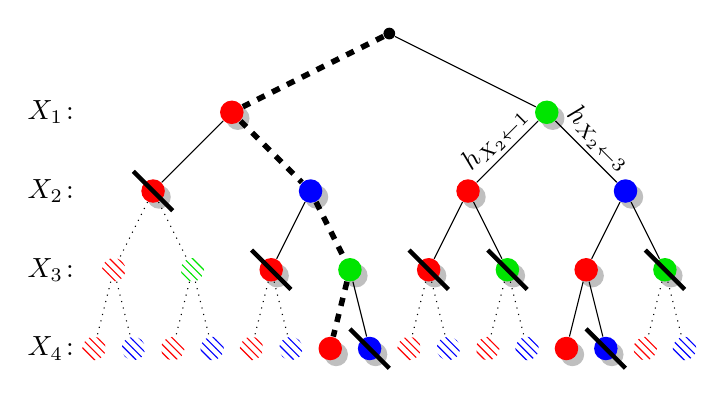
\begin{tikzpicture}
 [labelNode/.style   = {inner sep=0pt},
  rootNode/.style    = {circle, fill, inner sep=1.5pt},
  redNode/.style     = {circle, fill, inner sep=3pt, drop shadow,
                        red},
  greenNode/.style   = {circle, fill, inner sep=3pt, drop shadow,
                        green!90!black},
  blueNode/.style    = {circle, fill, inner sep=3pt, drop shadow,
                        blue},
  redPruned/.style   = {circle, fill, inner sep=3pt,
                        pattern=north west lines,
                        pattern color=red},
  greenPruned/.style = {circle, fill, inner sep=3pt,
                        pattern=north west lines,
                        pattern color=green!90!black},
  bluePruned/.style  = {circle, fill, inner sep=3pt,
                        pattern=north west lines,
                        pattern color=blue},
  pruned/.style = {dotted},
  solution/.style  = {line width=2pt, dashed}]
 %
 \node at (0,0) [rootNode] (root) {};
 %
 \node at (-4.3,-1) [labelNode]   {$X_1 \! :$};
 \node at (-2,  -1) [redNode]     (R)    {};
 \node at (+2,  -1) [greenNode]   (G)    {};
 %
 \node at (-4.3,-2) [labelNode]   {$X_2 \! :$};
 \node at (-3,  -2) [redNode]     (RR)   {};
  \draw [ultra thick] (-3.25,-1.75) -- (-2.75,-2.25);
 \node at (-1,  -2) [blueNode]    (RB)   {};
 \node at (+1,  -2) [redNode]     (GR)   {};
 \node at (+3,  -2) [blueNode]    (GB)   {};
 %
 \node at (-4.3,-3) [labelNode]   {$X_3 \! :$};
 \node at (-3.5,-3) [redPruned]   (RRR)  {};
 \node at (-2.5,-3) [greenPruned] (RRG)  {};
 \node at (-1.5,-3) [redNode]     (RBR)  {};
  \draw [ultra thick] (-1.75,-2.75) -- (-1.25,-3.25);
 \node at (-0.5,-3) [greenNode]   (RBG)  {};
 \node at (+0.5,-3) [redNode]     (GRR)  {};
  \draw [ultra thick] (+0.25,-2.75) -- (+0.75,-3.25);
 \node at (+1.5,-3) [greenNode]   (GRG)  {};
  \draw [ultra thick] (+1.25,-2.75) -- (+1.75,-3.25);
 \node at (+2.5,-3) [redNode]     (GBR)  {};
 \node at (+3.5,-3) [greenNode]   (GBG)  {};
  \draw [ultra thick] (+3.25,-2.75) -- (+3.75,-3.25);
 %
 \node at (-4.3, -4) [labelNode]  {$X_4 \! :$};
 \node at (-3.75,-4) [redPruned]  (RRRR) {};
 \node at (-3.25,-4) [bluePruned] (RRRB) {};
 \node at (-2.75,-4) [redPruned]  (RRGR) {};
 \node at (-2.25,-4) [bluePruned] (RRGB) {};
 \node at (-1.75,-4) [redPruned]  (RBRR) {};
 \node at (-1.25,-4) [bluePruned] (RBRB) {};
 \node at (-0.75,-4) [redNode]    (RBGR) {};
 \node at (-0.25,-4) [blueNode]   (RBGB) {};
  \draw [ultra thick] (-0.5,-3.75) -- (0,-4.25);
 \node at (+0.25,-4) [redPruned]  (GRRR) {};
 \node at (+0.75,-4) [bluePruned] (GRRB) {};
 \node at (+1.25,-4) [redPruned]  (GRGR) {};
 \node at (+1.75,-4) [bluePruned] (GRGB) {};
 \node at (+2.25,-4) [redNode]    (GBRR) {};
 \node at (+2.75,-4) [blueNode]   (GBRB) {};
  \draw [ultra thick] (+2.5,-3.75) -- (+3,-4.25);
 \node at (+3.25,-4) [redPruned]  (GBGR) {};
 \node at (+3.75,-4) [bluePruned] (GBGB) {};
 %
 \path
    (root)  edge [solution]  (R)
    (root)  edge  (G)
    %
    (R)     edge  (RR)
    (R)     edge [solution]  (RB)
    (G)     edge node [sloped,above=-2pt] {$h_{X_2 \gets 1}$} (GR)
    (G)     edge node [sloped,above=-2pt] {$h_{X_2 \gets 3}$} (GB)
    %
    (RR)    edge [pruned]  (RRR)
    (RR)    edge [pruned]  (RRG)
    (RB)    edge  (RBR)
    (RB)    edge [solution]  (RBG)
    (GR)    edge  (GRR)
    (GR)    edge  (GRG)
    (GB)    edge  (GBR)
    (GB)    edge  (GBG)
    %
    (RRR)   edge [pruned]  (RRRR)
    (RRR)   edge [pruned]  (RRRB)
    (RRG)   edge [pruned]  (RRGR)
    (RRG)   edge [pruned]  (RRGB)
    (RBR)   edge [pruned]  (RBRR)
    (RBR)   edge [pruned]  (RBRB)
    (RBG)   edge [solution]  (RBGR)
    (RBG)   edge  (RBGB)
    (GRR)   edge [pruned]  (GRRR)
    (GRR)   edge [pruned]  (GRRB)
    (GRG)   edge [pruned]  (GRGR)
    (GRG)   edge [pruned]  (GRGB)
    (GBR)   edge  (GBRR)
    (GBR)   edge  (GBRB)
    (GBG)   edge [pruned]  (GBGR)
    (GBG)   edge [pruned]  (GBGB)
    ;
\end{tikzpicture}
\caption{The search tree for
         Thessaly-coloring\label{pruned-tree}}
\end{figure}

\subsection{Heuristics exploitation in related work}

In \emph{constructive search,} one can build a solution
either with a deterministic\slash systematic search method,
or by making one-by-one random assignments. Do these methods
exploit heuristics and how?

\subsubsection{Deterministic search
               methods\label{deterministic}}

To our knowledge, existing search methods such as
\emph{limited discrepancy search} (LDS) use heuristics only
to \emph{order} the possible assignments and do not exploit
the \emph{difference} of the one heuristic estimation to
another, but only their \emph{rank}.\cite{lds} For example,
the \emph{iterative broadening} method explores only a
limited children's number for each search tree
node.\cite{ibroad} Of course, it chooses to visit only the
children with the highest ranks. \emph{Credit
search}\cite{dbs} and \emph{limited assignment number}
(LAN)\cite{lan} are other deterministic methods that also
take into account the rank of the heuristic estimations and
not the heuristic values themselves.

Last but not least, there are also methods that make the
assumption that \emph{the heuristic function is more
reliable as the search tree node depth increases.} E.g.,
\emph{depth-bounded discrepancy search} (DDS) allows to
override a heuristic estimation, only when we have not yet
reached a specific search tree depth.\cite{dds} Finally,
there are some methodologies that take into account two or
more heuristic functions and \emph{learn} as the search
proceeds, which heuristic is the best to use.\cite{learn}

\subsubsection{Random search methods\label{random}}

On the other hand, stochastic search methods completely
ignore heuristics, as they choose to make an assignment at
random.\cite{heuristics} For example, \emph{depth first
search with restarts} traverses the search tree making
random choices, and when a specific time limit is reached,
it re-starts from the beginning.

\subsubsection{Heuristics and probabilities}

Thus, the well-known search methods either use heuristics as
$\mathsf{Choices}$ ranks, or completely ignore them. In
1996, Bresina transformed the heuristic ranks into
\emph{probabilities} via the so-called
\emph{heuristic-biased stochastic sampling}
(HBSS).\cite{bresina-hbss} He provided a set of various
decreasing functions $\mathsf{bias}(r)$, e.g.\ $\frac{1}{r}$
or $e^{-r}$ etc., that take a specific integer choice rank
$r \in \{1, 2, \ldots\}$ and return a number that
corresponds to the probability of the choice to be selected.
Cicirello and Smith improved HBSS by introducing the
\emph{value-biased stochastic sampling} (VBSS). The
$\mathsf{bias}$ function now takes as argument the heuristic
\emph{value} itself.\cite{cicirello-vbss}

On the other hand, Gomes et al.\ exploit the so-called
\emph{heuristic-equivalence} to equate the choices with the
highest heuristic values. In this way, we can exclude the
choices with the lower heuristic values and select at random
amongst the choices with the most prevailing
values.\cite{equivalence}

\begin{figure}
\centering
% GNUPLOT: LaTeX picture with Postscript
\begingroup
  \makeatletter
  \providecommand\color[2][]{%
    \GenericError{(gnuplot) \space\space\space\@spaces}{%
      Package color not loaded in conjunction with
      terminal option `colourtext'%
    }{See the gnuplot documentation for explanation.%
    }{Either use 'blacktext' in gnuplot or load the package
      color.sty in LaTeX.}%
    \renewcommand\color[2][]{}%
  }%
  \providecommand\includegraphics[2][]{%
    \GenericError{(gnuplot) \space\space\space\@spaces}{%
      Package graphicx or graphics not loaded%
    }{See the gnuplot documentation for explanation.%
    }{The gnuplot epslatex terminal needs graphicx.sty or graphics.sty.}%
    \renewcommand\includegraphics[2][]{}%
  }%
  \providecommand\rotatebox[2]{#2}%
  \@ifundefined{ifGPcolor}{%
    \newif\ifGPcolor
    \GPcolortrue
  }{}%
  \@ifundefined{ifGPblacktext}{%
    \newif\ifGPblacktext
    \GPblacktexttrue
  }{}%
  % define a \g@addto@macro without @ in the name:
  \let\gplgaddtomacro\g@addto@macro
  % define empty templates for all commands taking text:
  \gdef\gplbacktext{}%
  \gdef\gplfronttext{}%
  \makeatother
  \ifGPblacktext
    % no textcolor at all
    \def\colorrgb#1{}%
    \def\colorgray#1{}%
  \else
    % gray or color?
    \ifGPcolor
      \def\colorrgb#1{\color[rgb]{#1}}%
      \def\colorgray#1{\color[gray]{#1}}%
      \expandafter\def\csname LTw\endcsname{\color{white}}%
      \expandafter\def\csname LTb\endcsname{\color{black}}%
      \expandafter\def\csname LTa\endcsname{\color{black}}%
      \expandafter\def\csname LT0\endcsname{\color[rgb]{1,0,0}}%
      \expandafter\def\csname LT1\endcsname{\color[rgb]{0,1,0}}%
      \expandafter\def\csname LT2\endcsname{\color[rgb]{0,0,1}}%
      \expandafter\def\csname LT3\endcsname{\color[rgb]{1,0,1}}%
      \expandafter\def\csname LT4\endcsname{\color[rgb]{0,1,1}}%
      \expandafter\def\csname LT5\endcsname{\color[rgb]{1,1,0}}%
      \expandafter\def\csname LT6\endcsname{\color[rgb]{0,0,0}}%
      \expandafter\def\csname LT7\endcsname{\color[rgb]{1,0.3,0}}%
      \expandafter\def\csname LT8\endcsname{\color[rgb]{0.5,0.5,0.5}}%
    \else
      % gray
      \def\colorrgb#1{\color{black}}%
      \def\colorgray#1{\color[gray]{#1}}%
      \expandafter\def\csname LTw\endcsname{\color{white}}%
      \expandafter\def\csname LTb\endcsname{\color{black}}%
      \expandafter\def\csname LTa\endcsname{\color{black}}%
      \expandafter\def\csname LT0\endcsname{\color{black}}%
      \expandafter\def\csname LT1\endcsname{\color{black}}%
      \expandafter\def\csname LT2\endcsname{\color{black}}%
      \expandafter\def\csname LT3\endcsname{\color{black}}%
      \expandafter\def\csname LT4\endcsname{\color{black}}%
      \expandafter\def\csname LT5\endcsname{\color{black}}%
      \expandafter\def\csname LT6\endcsname{\color{black}}%
      \expandafter\def\csname LT7\endcsname{\color{black}}%
      \expandafter\def\csname LT8\endcsname{\color{black}}%
    \fi
  \fi
  \setlength{\unitlength}{0.0500bp}%
  \begin{picture}(4824.00,2016.00)%
    \gplgaddtomacro\gplbacktext{%
      \csname LTb\endcsname%
      \put(550,440){\makebox(0,0)[r]{\strut{}$\scriptstyle{0}$}}%
      \put(550,679){\makebox(0,0)[r]{\strut{}$\scriptstyle{1}$}}%
      \put(550,917){\makebox(0,0)[r]{\strut{}$\scriptstyle{2}$}}%
      \put(550,1156){\makebox(0,0)[r]{\strut{}$\scriptstyle{3}$}}%
      \put(550,1394){\makebox(0,0)[r]{\strut{}$\scriptstyle{4}$}}%
      \put(550,1633){\makebox(0,0)[r]{\strut{}$\scriptstyle{5}$}}%
      \put(1057,220){\makebox(0,0){\strut{}$v_1$}}%
      \put(1806,220){\makebox(0,0){\strut{}$v_2$}}%
      \put(2555,220){\makebox(0,0){\strut{}$v_3$}}%
      \put(3304,220){\makebox(0,0){\strut{}$v_4$}}%
      \put(4053,220){\makebox(0,0){\strut{}$v_5$}}%
      \put(176,1096){\rotatebox{-270}{\makebox(0,0){\strut{}$h_i$}}}%
    }%
    \gplgaddtomacro\gplfronttext{%
    }%
    \gplbacktext
    \put(0,0){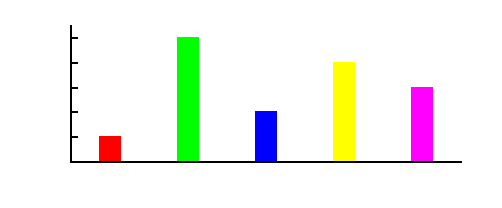
\includegraphics{heuristics}}%
    \gplfronttext
  \end{picture}%
\endgroup

\caption{Heuristic estimations $h_i$ for each value $v_i$\label{heuristics}}
\end{figure}

\begin{figure}
\centering
% GNUPLOT: LaTeX picture with Postscript
\begingroup
  \makeatletter
  \providecommand\color[2][]{%
    \GenericError{(gnuplot) \space\space\space\@spaces}{%
      Package color not loaded in conjunction with
      terminal option `colourtext'%
    }{See the gnuplot documentation for explanation.%
    }{Either use 'blacktext' in gnuplot or load the package
      color.sty in LaTeX.}%
    \renewcommand\color[2][]{}%
  }%
  \providecommand\includegraphics[2][]{%
    \GenericError{(gnuplot) \space\space\space\@spaces}{%
      Package graphicx or graphics not loaded%
    }{See the gnuplot documentation for explanation.%
    }{The gnuplot epslatex terminal needs graphicx.sty or graphics.sty.}%
    \renewcommand\includegraphics[2][]{}%
  }%
  \providecommand\rotatebox[2]{#2}%
  \@ifundefined{ifGPcolor}{%
    \newif\ifGPcolor
    \GPcolortrue
  }{}%
  \@ifundefined{ifGPblacktext}{%
    \newif\ifGPblacktext
    \GPblacktexttrue
  }{}%
  % define a \g@addto@macro without @ in the name:
  \let\gplgaddtomacro\g@addto@macro
  % define empty templates for all commands taking text:
  \gdef\gplbacktext{}%
  \gdef\gplfronttext{}%
  \makeatother
  \ifGPblacktext
    % no textcolor at all
    \def\colorrgb#1{}%
    \def\colorgray#1{}%
  \else
    % gray or color?
    \ifGPcolor
      \def\colorrgb#1{\color[rgb]{#1}}%
      \def\colorgray#1{\color[gray]{#1}}%
      \expandafter\def\csname LTw\endcsname{\color{white}}%
      \expandafter\def\csname LTb\endcsname{\color{black}}%
      \expandafter\def\csname LTa\endcsname{\color{black}}%
      \expandafter\def\csname LT0\endcsname{\color[rgb]{1,0,0}}%
      \expandafter\def\csname LT1\endcsname{\color[rgb]{0,1,0}}%
      \expandafter\def\csname LT2\endcsname{\color[rgb]{0,0,1}}%
      \expandafter\def\csname LT3\endcsname{\color[rgb]{1,0,1}}%
      \expandafter\def\csname LT4\endcsname{\color[rgb]{0,1,1}}%
      \expandafter\def\csname LT5\endcsname{\color[rgb]{1,1,0}}%
      \expandafter\def\csname LT6\endcsname{\color[rgb]{0,0,0}}%
      \expandafter\def\csname LT7\endcsname{\color[rgb]{1,0.3,0}}%
      \expandafter\def\csname LT8\endcsname{\color[rgb]{0.5,0.5,0.5}}%
    \else
      % gray
      \def\colorrgb#1{\color{black}}%
      \def\colorgray#1{\color[gray]{#1}}%
      \expandafter\def\csname LTw\endcsname{\color{white}}%
      \expandafter\def\csname LTb\endcsname{\color{black}}%
      \expandafter\def\csname LTa\endcsname{\color{black}}%
      \expandafter\def\csname LT0\endcsname{\color{black}}%
      \expandafter\def\csname LT1\endcsname{\color{black}}%
      \expandafter\def\csname LT2\endcsname{\color{black}}%
      \expandafter\def\csname LT3\endcsname{\color{black}}%
      \expandafter\def\csname LT4\endcsname{\color{black}}%
      \expandafter\def\csname LT5\endcsname{\color{black}}%
      \expandafter\def\csname LT6\endcsname{\color{black}}%
      \expandafter\def\csname LT7\endcsname{\color{black}}%
      \expandafter\def\csname LT8\endcsname{\color{black}}%
    \fi
  \fi
  \setlength{\unitlength}{0.0500bp}%
  \begin{picture}(4824.00,2016.00)%
    \gplgaddtomacro\gplbacktext{%
      \csname LTb\endcsname%
      \put(726,440){\makebox(0,0)[r]{\strut{}$\scriptstyle{0}$}}%
      \put(726,679){\makebox(0,0)[r]{\strut{}$\scriptstyle{0.2}$}}%
      \put(726,917){\makebox(0,0)[r]{\strut{}$\scriptstyle{0.4}$}}%
      \put(726,1156){\makebox(0,0)[r]{\strut{}$\scriptstyle{0.6}$}}%
      \put(726,1394){\makebox(0,0)[r]{\strut{}$\scriptstyle{0.8}$}}%
      \put(726,1633){\makebox(0,0)[r]{\strut{}$\scriptstyle{1}$}}%
      \put(1215,220){\makebox(0,0){\strut{}$v_1$}}%
      \put(1929,220){\makebox(0,0){\strut{}$v_2$}}%
      \put(2642,220){\makebox(0,0){\strut{}$v_3$}}%
      \put(3356,220){\makebox(0,0){\strut{}$v_4$}}%
      \put(4070,220){\makebox(0,0){\strut{}$v_5$}}%
      \put(220,1096){\rotatebox{-270}{\makebox(0,0){\strut{}$P(i)$}}}%
    }%
    \gplgaddtomacro\gplfronttext{%
    }%
    \gplbacktext
    \put(0,0){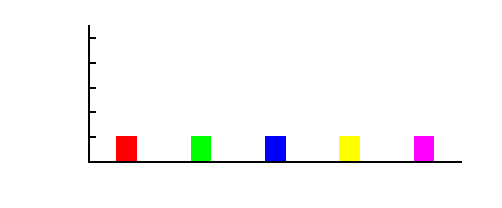
\includegraphics{uniform}}%
    \gplfronttext
  \end{picture}%
\endgroup

\caption{The probability is spread uniformly\label{uniform}}
\end{figure}

\begin{figure}
\centering
% GNUPLOT: LaTeX picture with Postscript
\begingroup
  \makeatletter
  \providecommand\color[2][]{%
    \GenericError{(gnuplot) \space\space\space\@spaces}{%
      Package color not loaded in conjunction with
      terminal option `colourtext'%
    }{See the gnuplot documentation for explanation.%
    }{Either use 'blacktext' in gnuplot or load the package
      color.sty in LaTeX.}%
    \renewcommand\color[2][]{}%
  }%
  \providecommand\includegraphics[2][]{%
    \GenericError{(gnuplot) \space\space\space\@spaces}{%
      Package graphicx or graphics not loaded%
    }{See the gnuplot documentation for explanation.%
    }{The gnuplot epslatex terminal needs graphicx.sty or graphics.sty.}%
    \renewcommand\includegraphics[2][]{}%
  }%
  \providecommand\rotatebox[2]{#2}%
  \@ifundefined{ifGPcolor}{%
    \newif\ifGPcolor
    \GPcolortrue
  }{}%
  \@ifundefined{ifGPblacktext}{%
    \newif\ifGPblacktext
    \GPblacktexttrue
  }{}%
  % define a \g@addto@macro without @ in the name:
  \let\gplgaddtomacro\g@addto@macro
  % define empty templates for all commands taking text:
  \gdef\gplbacktext{}%
  \gdef\gplfronttext{}%
  \makeatother
  \ifGPblacktext
    % no textcolor at all
    \def\colorrgb#1{}%
    \def\colorgray#1{}%
  \else
    % gray or color?
    \ifGPcolor
      \def\colorrgb#1{\color[rgb]{#1}}%
      \def\colorgray#1{\color[gray]{#1}}%
      \expandafter\def\csname LTw\endcsname{\color{white}}%
      \expandafter\def\csname LTb\endcsname{\color{black}}%
      \expandafter\def\csname LTa\endcsname{\color{black}}%
      \expandafter\def\csname LT0\endcsname{\color[rgb]{1,0,0}}%
      \expandafter\def\csname LT1\endcsname{\color[rgb]{0,1,0}}%
      \expandafter\def\csname LT2\endcsname{\color[rgb]{0,0,1}}%
      \expandafter\def\csname LT3\endcsname{\color[rgb]{1,0,1}}%
      \expandafter\def\csname LT4\endcsname{\color[rgb]{0,1,1}}%
      \expandafter\def\csname LT5\endcsname{\color[rgb]{1,1,0}}%
      \expandafter\def\csname LT6\endcsname{\color[rgb]{0,0,0}}%
      \expandafter\def\csname LT7\endcsname{\color[rgb]{1,0.3,0}}%
      \expandafter\def\csname LT8\endcsname{\color[rgb]{0.5,0.5,0.5}}%
    \else
      % gray
      \def\colorrgb#1{\color{black}}%
      \def\colorgray#1{\color[gray]{#1}}%
      \expandafter\def\csname LTw\endcsname{\color{white}}%
      \expandafter\def\csname LTb\endcsname{\color{black}}%
      \expandafter\def\csname LTa\endcsname{\color{black}}%
      \expandafter\def\csname LT0\endcsname{\color{black}}%
      \expandafter\def\csname LT1\endcsname{\color{black}}%
      \expandafter\def\csname LT2\endcsname{\color{black}}%
      \expandafter\def\csname LT3\endcsname{\color{black}}%
      \expandafter\def\csname LT4\endcsname{\color{black}}%
      \expandafter\def\csname LT5\endcsname{\color{black}}%
      \expandafter\def\csname LT6\endcsname{\color{black}}%
      \expandafter\def\csname LT7\endcsname{\color{black}}%
      \expandafter\def\csname LT8\endcsname{\color{black}}%
    \fi
  \fi
  \setlength{\unitlength}{0.0500bp}%
  \begin{picture}(4824.00,2016.00)%
    \gplgaddtomacro\gplbacktext{%
      \csname LTb\endcsname%
      \put(726,440){\makebox(0,0)[r]{\strut{}$\scriptstyle{0}$}}%
      \put(726,679){\makebox(0,0)[r]{\strut{}$\scriptstyle{0.2}$}}%
      \put(726,917){\makebox(0,0)[r]{\strut{}$\scriptstyle{0.4}$}}%
      \put(726,1156){\makebox(0,0)[r]{\strut{}$\scriptstyle{0.6}$}}%
      \put(726,1394){\makebox(0,0)[r]{\strut{}$\scriptstyle{0.8}$}}%
      \put(726,1633){\makebox(0,0)[r]{\strut{}$\scriptstyle{1}$}}%
      \put(1215,220){\makebox(0,0){\strut{}$v_1$}}%
      \put(1929,220){\makebox(0,0){\strut{}$v_2$}}%
      \put(2642,220){\makebox(0,0){\strut{}$v_3$}}%
      \put(3356,220){\makebox(0,0){\strut{}$v_4$}}%
      \put(4070,220){\makebox(0,0){\strut{}$v_5$}}%
      \put(220,1096){\rotatebox{-270}{\makebox(0,0){\strut{}$P(i)$}}}%
    }%
    \gplgaddtomacro\gplfronttext{%
    }%
    \gplbacktext
    \put(0,0){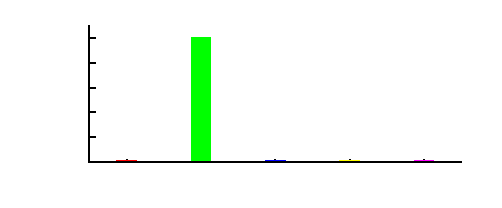
\includegraphics{systematic}}%
    \gplfronttext
  \end{picture}%
\endgroup

\caption{Systematic search favours the highest $h_i$\label{systematic}}
\end{figure}

\begin{figure}
\centering
% GNUPLOT: LaTeX picture with Postscript
\begingroup
  \makeatletter
  \providecommand\color[2][]{%
    \GenericError{(gnuplot) \space\space\space\@spaces}{%
      Package color not loaded in conjunction with
      terminal option `colourtext'%
    }{See the gnuplot documentation for explanation.%
    }{Either use 'blacktext' in gnuplot or load the package
      color.sty in LaTeX.}%
    \renewcommand\color[2][]{}%
  }%
  \providecommand\includegraphics[2][]{%
    \GenericError{(gnuplot) \space\space\space\@spaces}{%
      Package graphicx or graphics not loaded%
    }{See the gnuplot documentation for explanation.%
    }{The gnuplot epslatex terminal needs graphicx.sty or graphics.sty.}%
    \renewcommand\includegraphics[2][]{}%
  }%
  \providecommand\rotatebox[2]{#2}%
  \@ifundefined{ifGPcolor}{%
    \newif\ifGPcolor
    \GPcolortrue
  }{}%
  \@ifundefined{ifGPblacktext}{%
    \newif\ifGPblacktext
    \GPblacktexttrue
  }{}%
  % define a \g@addto@macro without @ in the name:
  \let\gplgaddtomacro\g@addto@macro
  % define empty templates for all commands taking text:
  \gdef\gplbacktext{}%
  \gdef\gplfronttext{}%
  \makeatother
  \ifGPblacktext
    % no textcolor at all
    \def\colorrgb#1{}%
    \def\colorgray#1{}%
  \else
    % gray or color?
    \ifGPcolor
      \def\colorrgb#1{\color[rgb]{#1}}%
      \def\colorgray#1{\color[gray]{#1}}%
      \expandafter\def\csname LTw\endcsname{\color{white}}%
      \expandafter\def\csname LTb\endcsname{\color{black}}%
      \expandafter\def\csname LTa\endcsname{\color{black}}%
      \expandafter\def\csname LT0\endcsname{\color[rgb]{1,0,0}}%
      \expandafter\def\csname LT1\endcsname{\color[rgb]{0,1,0}}%
      \expandafter\def\csname LT2\endcsname{\color[rgb]{0,0,1}}%
      \expandafter\def\csname LT3\endcsname{\color[rgb]{1,0,1}}%
      \expandafter\def\csname LT4\endcsname{\color[rgb]{0,1,1}}%
      \expandafter\def\csname LT5\endcsname{\color[rgb]{1,1,0}}%
      \expandafter\def\csname LT6\endcsname{\color[rgb]{0,0,0}}%
      \expandafter\def\csname LT7\endcsname{\color[rgb]{1,0.3,0}}%
      \expandafter\def\csname LT8\endcsname{\color[rgb]{0.5,0.5,0.5}}%
    \else
      % gray
      \def\colorrgb#1{\color{black}}%
      \def\colorgray#1{\color[gray]{#1}}%
      \expandafter\def\csname LTw\endcsname{\color{white}}%
      \expandafter\def\csname LTb\endcsname{\color{black}}%
      \expandafter\def\csname LTa\endcsname{\color{black}}%
      \expandafter\def\csname LT0\endcsname{\color{black}}%
      \expandafter\def\csname LT1\endcsname{\color{black}}%
      \expandafter\def\csname LT2\endcsname{\color{black}}%
      \expandafter\def\csname LT3\endcsname{\color{black}}%
      \expandafter\def\csname LT4\endcsname{\color{black}}%
      \expandafter\def\csname LT5\endcsname{\color{black}}%
      \expandafter\def\csname LT6\endcsname{\color{black}}%
      \expandafter\def\csname LT7\endcsname{\color{black}}%
      \expandafter\def\csname LT8\endcsname{\color{black}}%
    \fi
  \fi
  \setlength{\unitlength}{0.0500bp}%
  \begin{picture}(4824.00,3376.80)%
    \gplgaddtomacro\gplbacktext{%
      \csname LTb\endcsname%
      \put(3466,711){\rotatebox{28}{\makebox(0,0)[l]{\strut{}$\mathsf{conf}$}}}%
    }%
    \gplgaddtomacro\gplfronttext{%
      \csname LTb\endcsname%
      \put(957,907){\makebox(0,0){\strut{}$v_1$}}%
      \put(1332,842){\makebox(0,0){\strut{}$v_2$}}%
      \put(1707,778){\makebox(0,0){\strut{}$v_3$}}%
      \put(2082,713){\makebox(0,0){\strut{}$v_4$}}%
      \put(2456,648){\makebox(0,0){\strut{}$v_5$}}%
      \put(2962,662){\makebox(0,0){\strut{}$\scriptstyle{0}$}}%
      \put(3200,785){\makebox(0,0){\strut{}$\scriptstyle{1}$}}%
      \put(3438,909){\makebox(0,0){\strut{}$\scriptstyle{2}$}}%
      \put(3676,1032){\makebox(0,0){\strut{}$\scriptstyle{3}$}}%
      \put(3915,1156){\makebox(0,0){\strut{}$\scriptstyle{4}$}}%
      \put(4153,1279){\makebox(0,0){\strut{}$\scriptstyle{5}$}}%
      \put(660,1051){\makebox(0,0)[r]{\strut{}$\scriptstyle{0}$}}%
      \put(660,1298){\makebox(0,0)[r]{\strut{}$\scriptstyle{0.2}$}}%
      \put(660,1545){\makebox(0,0)[r]{\strut{}$\scriptstyle{0.4}$}}%
      \put(660,1792){\makebox(0,0)[r]{\strut{}$\scriptstyle{0.6}$}}%
      \put(660,2037){\makebox(0,0)[r]{\strut{}$\scriptstyle{0.8}$}}%
      \put(660,2284){\makebox(0,0)[r]{\strut{}$\scriptstyle{1}$}}%
      \put(270,1757){\rotatebox{-270}{\makebox(0,0){\strut{}$P(i)$}}}%
    }%
    \gplbacktext
    \put(0,0){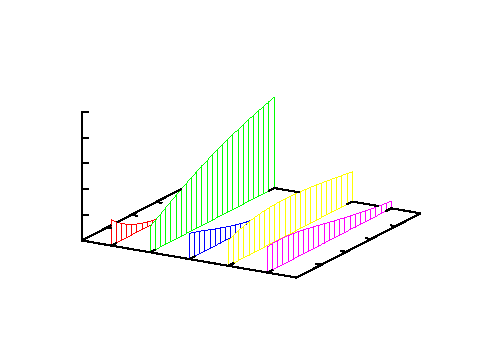
\includegraphics{conf}}%
    \gplfronttext
  \end{picture}%
\endgroup

\caption{As $\mathsf{conf}$ rises, the effect to $P(i)$ is greater\label{conf}}
\end{figure}


\section{New Probabilistic Heuristics}

Our contribution lies in the mathematical foundation of a framework that covers the above heuristic categories. In contrast to existing methodologies, we leverage on the \emph{smooth} transition from the total randomness to determinism.

%\subsection{Heuristics linearization}
%
%In order to assign a probability to a specific choice, its heuristic estimation must be a real number. This is not always the case, because in general, heuristics are vectors of positive real numbers.
%\begin{definition}
%A \emph{heuristic vector} $\mathbf{h} \in \mathbb{R}^n$ consists of multiple heuristic estimations. If $\mathbf{h} = [h_{x_1} \; h_{x_2} \; \cdots \; h_{x_n}]$, the $h_{x_1}$ is the \emph{primary heuristic estimation,} $h_{x_2}$ is the \emph{secondary heuristic estimation,} and $h_{x_n}$ is the \emph{$n$-ary heuristic estimation} for the same choice.
%\end{definition}
%\begin{property}
%A heuristic estimation $\mathbf{h_1}$ is stronger than $\mathbf{h_2}$, iff $\mathbf{h_1}$ is lexicographically greater than $\mathbf{h_2}$. In other words, the choice $1$ that corresponds to $\mathbf{h_1}$ is preferable to choice $2$, when $\mathbf{h_1} \succ_\mathrm{lex} \mathbf{h_2}$.
%\end{property}
%\begin{example}
%\label{vector}
%Let $\mathbf{h_a} = [7 \; 4 \; 8]$, $\mathbf{h_b} = [2 \; 5 \; 3]$, and $\mathbf{h_c} = [7 \; 9 \; 6]$. Heuristic $\mathbf{h_a}$ is stronger than $\mathbf{h_b}$, as it has a greater primary heuristic estimation ($7 > 2$). However, $\mathbf{h_a}$ is weaker than $\mathbf{h_c}$, as it has an equal primary heuristic estimation ($7 = 7$), but a smaller secondary ($4 < 9$).
%\end{example}
%An easy way to to make the vector $\mathbf{h}$ a simple real number, is to multiply each coordinate $h_{x_i}$ with a base $b_i$ and sum them all up.
%\begin{definition}
%\label{linearization}
%The \emph{linearization} of $\mathbf{h} = [h_{x_1} \; h_{x_2} \; \cdots \; h_{x_n}]$ equals to $\mathsf{linear} (\mathbf{h}) = h_{x_1} \cdot b_1 + h_{x_2} \cdot b_2 + \cdots + h_{x_n} \cdot b_n$, where $b_n = 1$, $b_{n-1} = b_n \! \cdot \! ( \max h_{x_n} + 1 )$, \ldots, $b_1 = b_2 \! \cdot \! ( \max h_{x_2} + 1 )$.
%\end{definition}
%\begin{example}
%Take the three vectors of Example~\ref{vector}. The maximum secondary heuristic estimation is $\max h_{x_2} = \max \{ 4, 5, 9 \} = 9$. The maximum tertiary heuristic estimation is $\max h_{x_3} = \max \{ 8, 3, 6 \} = 8$. Consequently, by applying Definition~\ref{linearization}, $b_3 = 1$, $b_2 = b_3 ( \max h_{x_3} + 1 ) = 1 (8 + 1) = 9$, and $b_1 = b_2 ( \max h_{x_2} + 1 ) = 9 (9 + 1) = 90$.
%
%Thus, the linearizations of the vectors are $\mathsf{linear} (\mathbf{h_a}) = 7 b_1 + 4 b_2 + 8 b_3 = 674$, $\mathsf{linear} (\mathbf{h_b}) = 2 b_1 + 5 b_2 + 3 b_3 = 228$, and $\mathsf{linear} (\mathbf{h_c}) = 7 b_1 + 9 b_2 + 6 b_3 = 717$.
%\end{example}
%\begin{proposition}
%It can be proven that $\mathbf{h_1}$ is stronger than $\mathbf{h_2}$, iff $\mathsf{linear} (\mathbf{h_1}) > \mathsf{linear} (\mathbf{h_2})$.
%\end{proposition}
%Having transformed heuristic vectors into plain real numbers, we can now use them as probabilities.

\subsection{Heuristics probabilistic foundations}

Probabilities are a more precise way to depict heuristics than orderings, because heuristics are actually \emph{estimations} whether a choice will guide us to a solution; they are not a strict quality rank.

\begin{definition}
\label{hdf}
A function $P: \mathsf{Choices} \to [0 \, , 1]\,,$ namely a \emph{heuristic distribution function,} maps each available choice to a corresponding probability, i.e.\ $P(i)$.
\end{definition}
\begin{property}
It should hold that $\sum_i P(i) = 1$, as $P$ denotes a probability for each $i \in \mathsf{Choices}$.
\end{property}
Regarding random search methods (Section~\ref{random}), the probability is distributed uniformly along the $\mathsf{Choices}$. Conclusively,
\begin{proposition}
\label{probability-random}
The heuristic distribution for a random method is always $P(i) = \frac{1}{|\mathsf{Choices}|}$, $\forall \, i$.
\end{proposition}
\begin{example}
\label{distribution}
Say that $\mathsf{Choices} = \{ v_1, v_2, \ldots, v_5 \}$. Every $v_i$ denotes a possible assignment. Furthermore, in a specific search tree node we can make five different assignments, and their corresponding heuristic estimations $h_i$ are $1$, $5$, $2$, $4$, $3$ respectively, as in Fig.~\ref{heuristics}.

Figure~\ref{uniform} depicts the corresponding heuristic distribution function for a random method, that is $P(i) = \nicefrac{1}{5}$, $\forall \, i$.
\end{example}
On the other extreme, deterministic search methods (Section~\ref{deterministic}) always select the choice $v_i$ that corresponds to the $h_i$ with the highest rank.
\begin{proposition}
\label{probability-deterministic}
Formally, in deterministic search methods, if $i = \arg\max_j h_j$, then $P(i) = 1$, otherwise $P(i) = 0$.
\end{proposition}
\begin{example}
The greatest heuristic value in Example~\ref{distribution} is $h_2 = 5$. Hence, a deterministic search method would select $v_2$ with a certain probability $P(v_2) = 1$. Consequently, the rest of the probabilities are zero, as in Fig.~\ref{systematic}.
\end{example}
If there is more than one maximum heuristic value, deterministic methods arbitrarily concern only one of them as maximum. To simplify the following equations we will make the assumption that there is only one maximum. Without loss of generality, we also assume that heuristic values are non-zero.

\subsection{Bridging the two opposites}

We extend our previous formulation of the heuristic distribution function (Definition~\ref{hdf}) in order to compromise random and deterministic methods. We introduce a parameter $\mathsf{conf} \in \mathbb{R}^+$, that signifies how much the heuristic estimations will be taken into account; it is the heuristic \emph{confidence.} This $\mathsf{conf}$idence pararameter is the basis to define the condition when a heuristic distribution function is ``balanced''.
\begin{definition}
\label{balanced}
A parameterized heuristic distribution function $P_\mathsf{conf} (i)$ is \emph{balanced} if and only if:
\begin{enumerate}
\item[1.]
$\forall \, i$,
${\displaystyle \lim_{\mathsf{conf} \to 0} }  \!\!
P_\mathsf{conf} (i) = \frac{1}{|\mathsf{Choices}|}$, and
%
\item[2a.]
if $i = \arg\max_j h_j$,
${\displaystyle \lim_{\mathsf{conf} \to \infty} }  \!\!\!\!
        P_\mathsf{conf} (i) = 1$,
%
\item[2b.]
otherwise,
${\displaystyle \lim_{\mathsf{conf} \to \infty} }  \!\!\!\!
        P_\mathsf{conf} (i) = 0 \,$.
\end{enumerate}
Moreover, the function $P_\mathsf{conf} (i)$ must be monotonic and continuous with respect to $\mathsf{conf}$ and for fixed $i$.
\end{definition}
Intuitively, $\mathsf{conf}$ is the link between random and deterministic search methods, as the above definition covers both Proposition~\ref{probability-random} when $\mathsf{conf} \to 0$ and Proposition~\ref{probability-deterministic} when $\mathsf{conf} \to \infty$. In other words, $\mathsf{conf}$ is the position along the random-deterministic axis.

What happens for intermediate $\mathsf{conf}$ values? This depends on the precise parameterized heuristic distribution function instance. We define the following function that gently scales randomness.
\begin{lemma}
\label{exponential}
The function $P_\mathsf{conf} (i) = \frac{h_i^\mathsf{conf}}{\sum_j h_j^\mathsf{conf}}$ is balanced.\footnote{For $\mathsf{conf} = 1$, the function $P_1 (i) = \frac{h_i}{\sum_j h_j}$ is equivalent to the \emph{fitness proportionate selection} function---resembling a \emph{roulette wheel}---that is used in Genetic Algorithms.\cite{roulette}}
\end{lemma}
\begin{proof}
We prove Definition~\ref{balanced} three requirements.
\begin{enumerate}
\item[1.]
${\displaystyle \lim_{\mathsf{conf} \to 0} }  \!\!  P_\mathsf{conf} (i) =
\frac{h_i^0}{\sum\limits_{j \in \mathsf{Choices}} \!\!\!\! h_j^0} =
\frac{1}{\sum\limits_{j \in \mathsf{Choices}} \!\!\!\!\! 1} =
\frac{1}{|\mathsf{Choices}|} \, $.
%
\vspace{0.3em}
%
\item[2a.]
Let $n = |\mathsf{Choices}|$. This number is bounded as the possible assignments in a CSP are a finite set. Thus, the distribution function can be analyzed as
\[
P_\mathsf{conf} (i) =
{\textstyle \frac{h_i^\mathsf{conf}}{\sum_j h_j^\mathsf{conf}} } =
{\textstyle \frac{h_i^\mathsf{conf}}{h_1^\mathsf{conf} + h_2^\mathsf{conf} + \cdots + h_{\max}^\mathsf{conf} + \cdots + h_n^\mathsf{conf}} } \, .
\]
Let $h_{\max}$ be the maximum $h_i$. If we divide by $h_{\max}^\mathsf{conf}$ both the nominator and denominator, we have
\begin{IEEEeqnarray}{rCl}
P_\mathsf{conf} (i)
&  =  &
{\textstyle \frac{\left(\frac{h_i}{h_{\max}}\right)^\mathsf{conf}}{\left(\frac{h_1}{h_{\max}}\right)^\mathsf{conf} + \cdots + 1 + \cdots + \left(\frac{h_n}{h_{\max}}\right)^\mathsf{conf}} }
\nonumber  \\
&  =  &
{\textstyle \frac{\left(\frac{h_i}{h_{\max}}\right)^\mathsf{conf}}{1 + \sum_{j \neq \max} \left(\frac{h_j}{h_{\max}}\right)^\mathsf{conf}} } \, .
\label{function}
\end{IEEEeqnarray}
Here, $\max$ is an abbreviation for $\arg\max_i h_i$. Therefore, $\forall \, j \neq \max$,
\begin{IEEEeqnarray}{rCl}
h_j < h_{\max}
& \  \Longrightarrow \  &
\frac{h_j}{h_{\max}} < 1
\  \Longrightarrow \  \nonumber  \\
&                       &
\!\!\!
{\displaystyle \lim_{\mathsf{conf} \to \infty}}
\left(\frac{h_j}{h_{\max}}\right)^\mathsf{conf} \!\!\! = 0 \, . \quad
\label{limit}
\end{IEEEeqnarray}
As a result from \eqref{function} and \eqref{limit},
\begin{IEEEeqnarray}{rCl}
\lim_{\mathsf{conf} \to \infty}  \!\!\!\!  P_\mathsf{conf} (i)
&  =  &
{\textstyle \frac{\lim_{\mathsf{conf} \to \infty} \left(\frac{h_i}{h_{\max}}\right)^\mathsf{conf}}{1 + \sum_{j \neq \max} \lim_{\mathsf{conf} \to \infty} \left(\frac{h_j}{h_{\max}}\right)^\mathsf{conf}} }
\nonumber  \\
&  =  &
\lim_{\mathsf{conf} \to \infty}
{\textstyle \left(\frac{h_i}{h_{\max}}\right)^\mathsf{conf} } .
\label{final-limit}
\end{IEEEeqnarray}
A direct derivation is that for $i = \max \equiv \arg\max_j h_j$, we have $\lim_{\mathsf{conf} \to \infty} P_\mathsf{conf} (\max) = 1$, which is the second prerequisite for a balanced function.
%
\vspace{0.3em}
%
\item[2b.]
Finally, the last prerequisite of Definition~\ref{balanced} involves $i \neq \max \Rightarrow h_i < h_{\max} \Rightarrow \frac{h_i}{h_{\max}} < 1$, which, combined with \eqref{final-limit}, gives $\lim_{\mathsf{conf} \to \infty} P_\mathsf{conf} (i) = 0$, which had to be demonstrated.
\end{enumerate}
\end{proof}
The above function (in Lemma~\ref{exponential}) is balanced and it also moves smoothly from the random extreme to the deterministic one, because it is a \emph{continuous} function, with regard to $\mathsf{conf} \in \mathbb{R}^+$.

Hence, the overall function is a transition from the total randomness to the almost total determinism. This is illustrated in the three-dimensional Fig.~\ref{conf}, which for $\mathsf{conf} = 0$, is equivalent to the two-dimensional Fig.~\ref{uniform}, and when $\mathsf{conf} \to \infty$, it is equivalent to Fig.~\ref{systematic}.


\section{Piece of Pie Search}

The probabilistic framework founded in the previous section, naturally complies with existing search methods; it affects only the heuristic function and not the methods themselves. But in order to fully exploit the introduced heuristics framework, we built the new constructive search method \emph{Piece of Pie Search} (\textsc{PoPS}).

\subsection{The algorithm's core}

Figure~\ref{PopsSample} describes \textsc{PopsSample}, which is the \textsc{PoPS} core. It is called inside \textsc{PoPS} in order to solve a CSP by providing a complete and valid $\mathsf{Assignments}$ set, which is initially empty.

\begin{figure}
\centering
\begin{algorithmic}
\Function{PopsSample}{$\mathsf{PieceToCover}, \mathsf{conf}$}
        \If {$\mathsf{Assignments}$ violate any constraint}
                \State  \Return failure
        \ElsIf {$\mathsf{Assignments}$ include every variable}
                \State  Record $\mathsf{Assignments}$ as solution
                \State  \Return success
        \EndIf
        \State  $X \, \gets \, \Call{VariablesOrderHeuristic}{\mathscr{X}}$
        \State  $D_{X_\mathrm{init}} \, \gets \, D_X$
        \State  $\mathsf{CoveredPiece} \, \gets \, 0$
        \While {$\mathsf{CoveredPiece} \, \leq \, \mathsf{PieceToCover}$}
                \State  $\mathsf{value} \, \gets \, \Call{ValuesOrderHeuristic}{D_X, \mathsf{conf}}$
                \State  $\mathsf{CoveredPiece} \, \gets \, \mathsf{CoveredPiece} \, + \, \frac{h_{X \gets \mathsf{value}}^\mathsf{conf}}{\sum_{v \in D_{X_\mathrm{init}}} h_{X \gets v}^\mathsf{conf}}$
                \State  Assign $\mathsf{value}$ to $X$ and add it to $\mathsf{Assignments}$
                \State  \Call{PopsSample}{$\mathsf{PieceToCover}, \, \mathsf{conf} \! + \! \frac{100 - \mathsf{conf}}{|\mathscr{X}|}$}
                \State  Undo the assignment
                \State  $D_X \, \gets \, D_X - \{\mathsf{value}\}$
        \EndWhile
        \State  $D_X \, \gets \, D_{X_\mathrm{init}}$
                \Comment{Restores initial domain}
        \State  \Return failure
                \Comment{All alternative values are exhausted}
\EndFunction
\end{algorithmic}
\caption{The recursive {\normalfont\textsc{PopsSample}} called by {\normalfont\textsc{PoPS}}\label{PopsSample}}
\end{figure}

In each \textsc{PopsSample} call we get an unassigned variable returned by the function \textsc{VariablesOrderHeuristic}($\mathscr{X}$), where $\mathscr{X}$ is the set of all the constrained variables. Then, it stores its domain $D_X$, in order to restore it in a future backtrack. All the above steps are common in constructive search methods.

The crucial and novel part of this function is inside the \textbf{while} iteration where we iterate through the different values in $D_X$. The call \textsc{ValuesOrderHeuristic}($D_X, \mathsf{conf}$) returns the best value out of $D_X$, according to the heuristic estimation, using the heuristic function in Lemma~\ref{exponential}.

Normal search methods, like Depth First Search (DFS), %Depth-bounded Backtrack Search (DBS),
Limited Discrepancy Search (LDS), and other known deterministic methods explore in their steps a specific \emph{number} of values in $D_X$ or every value in it (cf.\ Section~\ref{deterministic}). In \textsc{PopsSample}, we explore a specific \emph{subset} $D_X'$ of $D_X$, which corresponds to a proportion of the heuristics pie. The proportion is the argument $\mathsf{PieceToCover} \in [0,1]$. When $\mathsf{PieceToCover}$ becomes $1$, then \textsc{PopsSample} is a complete search method as it explores all the $D_X$ set values.
\begin{example}
Figure~\ref{piechart} demonstrates the heuristics pie for the Example~\ref{distribution}: Each $h_i$ corresponds to a value $v_i$ in $D_X$. In this case, a \textsc{PopsSample}$(0.5,1)$ invocation would explore half the pie. E.g., the choices that correspond to the heuristics $h_1^1 + h_2^1 + h_3^1$ or $h_2^1 + h_5^1$ make half the pie and more.
\end{example}
The exponent in the heuristic values has to do with the $\mathsf{conf}$idence semantics in our framework.

\begin{figure}
\centering
% GNUPLOT: LaTeX picture with Postscript
\begingroup
  \makeatletter
  \providecommand\color[2][]{%
    \GenericError{(gnuplot) \space\space\space\@spaces}{%
      Package color not loaded in conjunction with
      terminal option `colourtext'%
    }{See the gnuplot documentation for explanation.%
    }{Either use 'blacktext' in gnuplot or load the package
      color.sty in LaTeX.}%
    \renewcommand\color[2][]{}%
  }%
  \providecommand\includegraphics[2][]{%
    \GenericError{(gnuplot) \space\space\space\@spaces}{%
      Package graphicx or graphics not loaded%
    }{See the gnuplot documentation for explanation.%
    }{The gnuplot epslatex terminal needs graphicx.sty or graphics.sty.}%
    \renewcommand\includegraphics[2][]{}%
  }%
  \providecommand\rotatebox[2]{#2}%
  \@ifundefined{ifGPcolor}{%
    \newif\ifGPcolor
    \GPcolortrue
  }{}%
  \@ifundefined{ifGPblacktext}{%
    \newif\ifGPblacktext
    \GPblacktexttrue
  }{}%
  % define a \g@addto@macro without @ in the name:
  \let\gplgaddtomacro\g@addto@macro
  % define empty templates for all commands taking text:
  \gdef\gplbacktext{}%
  \gdef\gplfronttext{}%
  \makeatother
  \ifGPblacktext
    % no textcolor at all
    \def\colorrgb#1{}%
    \def\colorgray#1{}%
  \else
    % gray or color?
    \ifGPcolor
      \def\colorrgb#1{\color[rgb]{#1}}%
      \def\colorgray#1{\color[gray]{#1}}%
      \expandafter\def\csname LTw\endcsname{\color{white}}%
      \expandafter\def\csname LTb\endcsname{\color{black}}%
      \expandafter\def\csname LTa\endcsname{\color{black}}%
      \expandafter\def\csname LT0\endcsname{\color[rgb]{1,0,0}}%
      \expandafter\def\csname LT1\endcsname{\color[rgb]{0,1,0}}%
      \expandafter\def\csname LT2\endcsname{\color[rgb]{0,0,1}}%
      \expandafter\def\csname LT3\endcsname{\color[rgb]{1,0,1}}%
      \expandafter\def\csname LT4\endcsname{\color[rgb]{0,1,1}}%
      \expandafter\def\csname LT5\endcsname{\color[rgb]{1,1,0}}%
      \expandafter\def\csname LT6\endcsname{\color[rgb]{0,0,0}}%
      \expandafter\def\csname LT7\endcsname{\color[rgb]{1,0.3,0}}%
      \expandafter\def\csname LT8\endcsname{\color[rgb]{0.5,0.5,0.5}}%
    \else
      % gray
      \def\colorrgb#1{\color{black}}%
      \def\colorgray#1{\color[gray]{#1}}%
      \expandafter\def\csname LTw\endcsname{\color{white}}%
      \expandafter\def\csname LTb\endcsname{\color{black}}%
      \expandafter\def\csname LTa\endcsname{\color{black}}%
      \expandafter\def\csname LT0\endcsname{\color{black}}%
      \expandafter\def\csname LT1\endcsname{\color{black}}%
      \expandafter\def\csname LT2\endcsname{\color{black}}%
      \expandafter\def\csname LT3\endcsname{\color{black}}%
      \expandafter\def\csname LT4\endcsname{\color{black}}%
      \expandafter\def\csname LT5\endcsname{\color{black}}%
      \expandafter\def\csname LT6\endcsname{\color{black}}%
      \expandafter\def\csname LT7\endcsname{\color{black}}%
      \expandafter\def\csname LT8\endcsname{\color{black}}%
    \fi
  \fi
  \setlength{\unitlength}{0.0500bp}%
  \begin{picture}(3810.96,3376.80)%
    \gplgaddtomacro\gplbacktext{%
      \csname LTb\endcsname%
      \put(3276,1804){\makebox(0,0){\strut{}$P(1)$}}%
      \put(2057,2867){\makebox(0,0){\strut{}$P(2)$}}%
      \put(534,1804){\makebox(0,0){\strut{}$P(3)$}}%
      \put(1202,346){\makebox(0,0){\strut{}$P(4)$}}%
      \put(3041,719){\makebox(0,0){\strut{}$P(5)$}}%
    }%
    \gplgaddtomacro\gplfronttext{%
    }%
    \gplbacktext
    \put(0,0){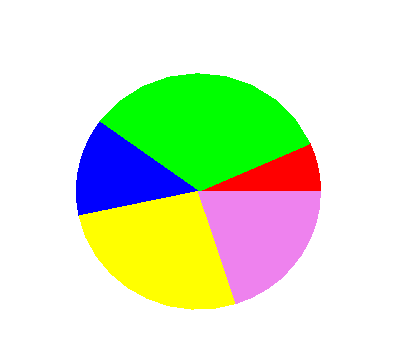
\includegraphics{piechart}}%
    \gplfronttext
  \end{picture}%
\endgroup

\caption{The heuristics pie chart for Example~\ref{distribution}\label{piechart}}
\end{figure}

\begin{figure}
\centering
\begin{algorithmic}
\Function{PoPS}{}
        \For {$i$ \textbf{from} $1$ \textbf{to} $\mathsf{SamplesNum}$}
                \State  $\mathsf{Sample}_i$ is activated
                \State  $\mathsf{Cover}_i \, \gets \, 0$
                \State  $\mathsf{conf}_i  \, \gets \, 100 \cdot \frac{i-1}{\mathsf{SamplesNum}-1}$
        \EndFor
        \While {the available time is not exhausted}
                \For {\textbf{each} active $\mathsf{Sample}_i$}
                        \If {\Call{PopsSample}{$\mathsf{Cover}_i, \mathsf{conf}_i$} \\
                        \hspace{5em} did not return a solution}
                                \State  $\mathsf{Sample}_i$ is deactivated
                        \EndIf
                        \State  $\mathsf{Cover}_i \, \gets \, \mathsf{Cover}_i + \frac{1}{d}$
                \EndFor
                \If  {every $\mathsf{Sample}_i$ is deactivated}
                        \State  Activate every $\mathsf{Sample}_i$
                        \Comment{to keep searching.}
                \EndIf
        \EndWhile
\EndFunction
\end{algorithmic}
\caption{Piece of Pie Search ({\normalfont\textsc{PoPS}}) Method\label{pops}}
\end{figure}

\subsection{Heuristic confidence vs.\ node level}

An important detail in \textsc{PopsSample} appearing in Fig.~\ref{PopsSample}, is the increase in $\mathsf{conf}$ as the current search tree node level deepens.

When we make the first recursive \textsc{PopsSample} call (inside \textbf{while}), we have already made an assignment. Hence, the current tree level will be augmented by $1$ and $\mathsf{conf}$ will be increased by $\frac{100 - \mathsf{conf}}{|\mathscr{X}|}$.

Each subsequent recursive call deepens search by $1$, until the current depth reaches $|\mathscr{X}|$, which means that every variable in $\mathscr{X}$ has been assigned a value. For a specific depth $k$ the $\mathsf{conf}$ value is increased by $k \cdot \frac{100 - \mathsf{conf}}{|\mathscr{X}|}$. Finally, when $k = |\mathscr{X}|$, the $\mathsf{conf}$ argument of \textsc{PopsSample} will become equal to the marginal value $100$.

In the deepest node levels, heuristics are usually more accurate, because even more variables have been instantiated and we have a clearer picture of the problem. In our framework, more accuracy means more confidence, that's why we increase $\mathsf{conf}$ as the search method proceeds with the assignments.

%\subsection{Computation of the covered piece of pie}
%
%A special detail is that in each iteration, $\frac{h_{X \gets \mathsf{value}}}{\sum_{v \in D_X} h_{X \gets v}}$ is added to the existing $\mathsf{CoveredPiece}$, multiplied by a factor $1.0 - \mathsf{CoveredPiece}$. Why is this factor needed?
%
%After each iteration, $D_X$ is shrunk, so the $\sum_{v \in D_X} h_{X \gets v}$ is altered. The \emph{initial} $D_X$ refers to the complete pie $1.0$, whilst the \emph{current} $D_X$ refers to the \emph{remaining} proportion of the overall piece, which is $1.0 - \mathsf{CoveredPiece}$.

\newcommand{\PoPS}{\textbf{\large P\normalsize O\large PS}}
\newcommand{\PopsSample}{\textbf{\large P\normalsize OPS\large S\normalsize AMPLE}}

\subsection{\PopsSample{} average complexity}

The \textsc{PopsSample} complexity depends on $\mathsf{PieceToCover}$ argument and the heuristic function distribution.
\begin{lemma}
Let $n$ be the constrained variables number and let $d$ be the average domain size. Then, the average complexity of a \textsc{PopsSample}$(\mathsf{PieceToCover},\mathsf{conf})$ call equals $\mathcal{O}(d^n \cdot \mathsf{PieceToCover}^n)$.
\end{lemma}
\begin{proof}
An initial \textsc{PopsSample}$(\mathsf{PieceToCover},\mathsf{conf})$ call, iterates through the values of, let's say, the first variable $X_1$. If the heuristic function numbers for the values in $D_{X_1}$ are uniformly distributed, the expected value for $h_{X_1 \gets \mathsf{value}}$ would be $\mu = \frac{\sum_{v \in D_{X_1}} h_{X \gets v}}{|D_{X_1}|}$.

Thus, to reach the pie proportion $A = \mathsf{PieceToCover} \cdot \sum_{v \in D_X} h_{X \gets v}$, we need $A / \mu = \mathsf{PieceToCover} \cdot |D_{X_1}|$ iterations, i.e.\ $\mathcal{O}(\mathsf{PieceToCover} \cdot d)$ loops.

The total time needed is $T_1 = \mathcal{O}(\mathsf{PieceToCover} \cdot d) \cdot T_2$, where $T_2$ is the time for the \textsc{PopsSample} call \emph{inside} the loop. It also holds that $T_2 = \mathcal{O}(\mathsf{PieceToCover} \cdot d) \cdot T_3$, etc., and finally $T_n = \mathcal{O}(\mathsf{PieceToCover} \cdot d)$. In conclusion, the aggregate complexity is $\mathcal{O}(\mathsf{PieceToCover}^n \cdot d^n)$ for the initial call.
\end{proof}
We can observe that \textsc{PopsSample}$(1,\mathsf{conf})$ is equivalent to a complete search space exploration, which has an $\mathcal{O}(d^n)$ time complexity.

\subsection{The motivation behind \PoPS\label{sampling}}

Finding the best $\mathsf{conf}$ is the motivation behind \textsc{PoPS}. Unfortunately, we do not know a priori which $\mathsf{conf}$ is the best parameter for \textsc{PopsSample}. However, we can find it by trial and error. In Fig.~\ref{pops}, the \textsc{PoPS} function invokes \textsc{PopsSample} for $\mathsf{SamplesNum}$ different $\mathsf{conf}_i$ values, including the marginal values $0$ and $100$.

Each different $\mathsf{conf}_i$ is used in turn. Initially, the $\mathsf{Cover}_i$ parameter in the \textsc{PoPS} algorithm is zero for every $\mathsf{conf}_i$. When a specific $\mathsf{conf}_i$ has been examined, the corresponding $\mathsf{Cover}_i$ is increased by $\frac{1}{d}$, where $d$ is the average domain size. When the second iteration over a specific $\mathsf{conf}_i$ ends, the $\mathsf{Cover}_i$ is increased again by $\frac{1}{d}$ and so on.

In this way, each $\mathsf{conf}_i$ is given the same opportunity (search space) to find a solution. If some $\mathsf{conf}_i$ does not produce a solution, it is deactivated. It is reactivated only if all other $\mathsf{conf}_i$'s fail to produce a solution.


\section{Empirical Evaluations}

The gradual switch from randomness to determinism can boost search in demanding CSPs, such as course scheduling and the radio frequency assignment problems. With the help of our free constraint programming C++ library \textsc{Naxos Solver},\cite{naxos-solver} we solved official instances of these problems for different heuristic distribution configurations.

The source code for our evaluations is freely available at \url{http://di.uoa.gr/~pothitos/PoPS} including the problem datasets. The experiments were conducted on an HP computer with an Intel dual-core E6750 processor clocked at 2.66\,GHz with 2\,GB of memory and a Xubuntu Linux 12.04 operating system.

For the following first three subsections, our $\mathsf{conf}$idence framework was used to randomize only the \emph{variables ordering heuristic} (minimum remaining values and degree used for tie breaking), whereas in the last subsection, which refers to \textsc{PoPS}, the randomization affects only the \textsc{ValuesOrderHeuristic} (least constraining value), called by \textsc{PopsSample} inside \textsc{PoPS}.

%For the first two subsections, the \emph{variables} ordering heuristic used is a mix of the selection of the variable with the \emph{minimum remaining values} (primary heuristic) and the variable having the maximum \emph{degree,} i.e.\ the variable connected to the greatest number of other variables (secondary heuristic). In the other two subsections, the \emph{values} ordering heuristic favours the \emph{least constraining values}, i.e.\ it gives a better heuristic estimation to the value that, if assigned, it will provoke the least domain restrictions to the other variables. Secondarily, it favours the value that, if assigned, it will contribute to the maximum improvement of the solution quality\slash cost (objective function).

%\cite{sabin-mace}
%\cite{handbook-cp}

\begin{figure}
\centering
% GNUPLOT: LaTeX picture with Postscript
\begingroup
  \makeatletter
  \providecommand\color[2][]{%
    \GenericError{(gnuplot) \space\space\space\@spaces}{%
      Package color not loaded in conjunction with
      terminal option `colourtext'%
    }{See the gnuplot documentation for explanation.%
    }{Either use 'blacktext' in gnuplot or load the package
      color.sty in LaTeX.}%
    \renewcommand\color[2][]{}%
  }%
  \providecommand\includegraphics[2][]{%
    \GenericError{(gnuplot) \space\space\space\@spaces}{%
      Package graphicx or graphics not loaded%
    }{See the gnuplot documentation for explanation.%
    }{The gnuplot epslatex terminal needs graphicx.sty or graphics.sty.}%
    \renewcommand\includegraphics[2][]{}%
  }%
  \providecommand\rotatebox[2]{#2}%
  \@ifundefined{ifGPcolor}{%
    \newif\ifGPcolor
    \GPcolortrue
  }{}%
  \@ifundefined{ifGPblacktext}{%
    \newif\ifGPblacktext
    \GPblacktexttrue
  }{}%
  % define a \g@addto@macro without @ in the name:
  \let\gplgaddtomacro\g@addto@macro
  % define empty templates for all commands taking text:
  \gdef\gplbacktext{}%
  \gdef\gplfronttext{}%
  \makeatother
  \ifGPblacktext
    % no textcolor at all
    \def\colorrgb#1{}%
    \def\colorgray#1{}%
  \else
    % gray or color?
    \ifGPcolor
      \def\colorrgb#1{\color[rgb]{#1}}%
      \def\colorgray#1{\color[gray]{#1}}%
      \expandafter\def\csname LTw\endcsname{\color{white}}%
      \expandafter\def\csname LTb\endcsname{\color{black}}%
      \expandafter\def\csname LTa\endcsname{\color{black}}%
      \expandafter\def\csname LT0\endcsname{\color[rgb]{1,0,0}}%
      \expandafter\def\csname LT1\endcsname{\color[rgb]{0,1,0}}%
      \expandafter\def\csname LT2\endcsname{\color[rgb]{0,0,1}}%
      \expandafter\def\csname LT3\endcsname{\color[rgb]{1,0,1}}%
      \expandafter\def\csname LT4\endcsname{\color[rgb]{0,1,1}}%
      \expandafter\def\csname LT5\endcsname{\color[rgb]{1,1,0}}%
      \expandafter\def\csname LT6\endcsname{\color[rgb]{0,0,0}}%
      \expandafter\def\csname LT7\endcsname{\color[rgb]{1,0.3,0}}%
      \expandafter\def\csname LT8\endcsname{\color[rgb]{0.5,0.5,0.5}}%
    \else
      % gray
      \def\colorrgb#1{\color{black}}%
      \def\colorgray#1{\color[gray]{#1}}%
      \expandafter\def\csname LTw\endcsname{\color{white}}%
      \expandafter\def\csname LTb\endcsname{\color{black}}%
      \expandafter\def\csname LTa\endcsname{\color{black}}%
      \expandafter\def\csname LT0\endcsname{\color{black}}%
      \expandafter\def\csname LT1\endcsname{\color{black}}%
      \expandafter\def\csname LT2\endcsname{\color{black}}%
      \expandafter\def\csname LT3\endcsname{\color{black}}%
      \expandafter\def\csname LT4\endcsname{\color{black}}%
      \expandafter\def\csname LT5\endcsname{\color{black}}%
      \expandafter\def\csname LT6\endcsname{\color{black}}%
      \expandafter\def\csname LT7\endcsname{\color{black}}%
      \expandafter\def\csname LT8\endcsname{\color{black}}%
    \fi
  \fi
  \setlength{\unitlength}{0.0500bp}%
  \begin{picture}(4824.00,3376.80)%
    \gplgaddtomacro\gplbacktext{%
      \csname LTb\endcsname%
      \put(726,704){\makebox(0,0)[r]{\strut{}$\scriptstyle{600}$}}%
      \put(726,1048){\makebox(0,0)[r]{\strut{}$\scriptstyle{650}$}}%
      \put(726,1392){\makebox(0,0)[r]{\strut{}$\scriptstyle{700}$}}%
      \put(726,1736){\makebox(0,0)[r]{\strut{}$\scriptstyle{750}$}}%
      \put(726,2080){\makebox(0,0)[r]{\strut{}$\scriptstyle{800}$}}%
      \put(726,2424){\makebox(0,0)[r]{\strut{}$\scriptstyle{850}$}}%
      \put(726,2768){\makebox(0,0)[r]{\strut{}$\scriptstyle{900}$}}%
      \put(726,3112){\makebox(0,0)[r]{\strut{}$\scriptstyle{950}$}}%
      \put(858,484){\makebox(0,0){\strut{}$\scriptstyle{0}$}}%
      \put(1368,484){\makebox(0,0){\strut{}$\scriptstyle{20}$}}%
      \put(1878,484){\makebox(0,0){\strut{}$\scriptstyle{40}$}}%
      \put(2388,484){\makebox(0,0){\strut{}$\scriptstyle{60}$}}%
      \put(2897,484){\makebox(0,0){\strut{}$\scriptstyle{80}$}}%
      \put(3407,484){\makebox(0,0){\strut{}$\scriptstyle{100}$}}%
      \put(3917,484){\makebox(0,0){\strut{}$\scriptstyle{120}$}}%
      \put(4427,484){\makebox(0,0){\strut{}$\scriptstyle{140}$}}%
      \put(220,1908){\rotatebox{-270}{\makebox(0,0){\strut{}Solution Cost}}}%
      \put(2642,154){\makebox(0,0){\strut{}$\mathsf{conf}$}}%
    }%
    \gplgaddtomacro\gplfronttext{%
      \csname LTb\endcsname%
      \put(3440,2950){\makebox(0,0)[r]{\strut{}\textsf{\scriptsize Ing0203-2}}}%
      \csname LTb\endcsname%
      \put(3440,2752){\makebox(0,0)[r]{\strut{}\textsf{\scriptsize Ing0304-1}}}%
      \csname LTb\endcsname%
      \put(3440,2554){\makebox(0,0)[r]{\strut{}\textsf{\scriptsize Ing0304-3}}}%
      \csname LTb\endcsname%
      \put(3440,2356){\makebox(0,0)[r]{\strut{}\textsf{\scriptsize Ing0405-2}}}%
      \csname LTb\endcsname%
      \put(3440,2158){\makebox(0,0)[r]{\strut{}\textsf{\scriptsize Ing0506-3}}}%
      \csname LTb\endcsname%
      \put(3440,1960){\makebox(0,0)[r]{\strut{}\textsf{\scriptsize Ing0708-1}}}%
    }%
    \gplbacktext
    \put(0,0){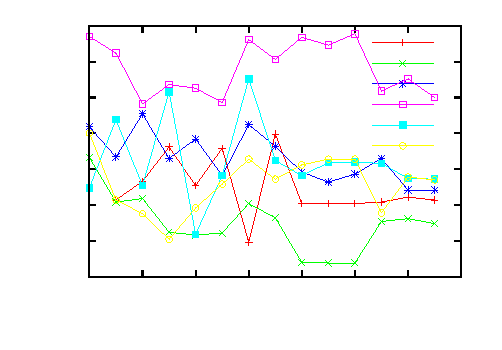
\includegraphics{costsA}}%
    \gplfronttext
  \end{picture}%
\endgroup

\caption{Timetabling solutions costs vs.\ $\mathsf{conf}$\label{costsA}}
\end{figure}

\begin{figure}
\centering
% GNUPLOT: LaTeX picture with Postscript
\begingroup
  \makeatletter
  \providecommand\color[2][]{%
    \GenericError{(gnuplot) \space\space\space\@spaces}{%
      Package color not loaded in conjunction with
      terminal option `colourtext'%
    }{See the gnuplot documentation for explanation.%
    }{Either use 'blacktext' in gnuplot or load the package
      color.sty in LaTeX.}%
    \renewcommand\color[2][]{}%
  }%
  \providecommand\includegraphics[2][]{%
    \GenericError{(gnuplot) \space\space\space\@spaces}{%
      Package graphicx or graphics not loaded%
    }{See the gnuplot documentation for explanation.%
    }{The gnuplot epslatex terminal needs graphicx.sty or graphics.sty.}%
    \renewcommand\includegraphics[2][]{}%
  }%
  \providecommand\rotatebox[2]{#2}%
  \@ifundefined{ifGPcolor}{%
    \newif\ifGPcolor
    \GPcolortrue
  }{}%
  \@ifundefined{ifGPblacktext}{%
    \newif\ifGPblacktext
    \GPblacktexttrue
  }{}%
  % define a \g@addto@macro without @ in the name:
  \let\gplgaddtomacro\g@addto@macro
  % define empty templates for all commands taking text:
  \gdef\gplbacktext{}%
  \gdef\gplfronttext{}%
  \makeatother
  \ifGPblacktext
    % no textcolor at all
    \def\colorrgb#1{}%
    \def\colorgray#1{}%
  \else
    % gray or color?
    \ifGPcolor
      \def\colorrgb#1{\color[rgb]{#1}}%
      \def\colorgray#1{\color[gray]{#1}}%
      \expandafter\def\csname LTw\endcsname{\color{white}}%
      \expandafter\def\csname LTb\endcsname{\color{black}}%
      \expandafter\def\csname LTa\endcsname{\color{black}}%
      \expandafter\def\csname LT0\endcsname{\color[rgb]{1,0,0}}%
      \expandafter\def\csname LT1\endcsname{\color[rgb]{0,1,0}}%
      \expandafter\def\csname LT2\endcsname{\color[rgb]{0,0,1}}%
      \expandafter\def\csname LT3\endcsname{\color[rgb]{1,0,1}}%
      \expandafter\def\csname LT4\endcsname{\color[rgb]{0,1,1}}%
      \expandafter\def\csname LT5\endcsname{\color[rgb]{1,1,0}}%
      \expandafter\def\csname LT6\endcsname{\color[rgb]{0,0,0}}%
      \expandafter\def\csname LT7\endcsname{\color[rgb]{1,0.3,0}}%
      \expandafter\def\csname LT8\endcsname{\color[rgb]{0.5,0.5,0.5}}%
    \else
      % gray
      \def\colorrgb#1{\color{black}}%
      \def\colorgray#1{\color[gray]{#1}}%
      \expandafter\def\csname LTw\endcsname{\color{white}}%
      \expandafter\def\csname LTb\endcsname{\color{black}}%
      \expandafter\def\csname LTa\endcsname{\color{black}}%
      \expandafter\def\csname LT0\endcsname{\color{black}}%
      \expandafter\def\csname LT1\endcsname{\color{black}}%
      \expandafter\def\csname LT2\endcsname{\color{black}}%
      \expandafter\def\csname LT3\endcsname{\color{black}}%
      \expandafter\def\csname LT4\endcsname{\color{black}}%
      \expandafter\def\csname LT5\endcsname{\color{black}}%
      \expandafter\def\csname LT6\endcsname{\color{black}}%
      \expandafter\def\csname LT7\endcsname{\color{black}}%
      \expandafter\def\csname LT8\endcsname{\color{black}}%
    \fi
  \fi
  \setlength{\unitlength}{0.0500bp}%
  \begin{picture}(4824.00,3376.80)%
    \gplgaddtomacro\gplbacktext{%
      \csname LTb\endcsname%
      \put(858,704){\makebox(0,0)[r]{\strut{}$\scriptstyle{0}$}}%
      \put(858,923){\makebox(0,0)[r]{\strut{}$\scriptstyle{200}$}}%
      \put(858,1142){\makebox(0,0)[r]{\strut{}$\scriptstyle{400}$}}%
      \put(858,1361){\makebox(0,0)[r]{\strut{}$\scriptstyle{600}$}}%
      \put(858,1580){\makebox(0,0)[r]{\strut{}$\scriptstyle{800}$}}%
      \put(858,1799){\makebox(0,0)[r]{\strut{}$\scriptstyle{1000}$}}%
      \put(858,2017){\makebox(0,0)[r]{\strut{}$\scriptstyle{1200}$}}%
      \put(858,2236){\makebox(0,0)[r]{\strut{}$\scriptstyle{1400}$}}%
      \put(858,2455){\makebox(0,0)[r]{\strut{}$\scriptstyle{1600}$}}%
      \put(858,2674){\makebox(0,0)[r]{\strut{}$\scriptstyle{1800}$}}%
      \put(858,2893){\makebox(0,0)[r]{\strut{}$\scriptstyle{2000}$}}%
      \put(858,3112){\makebox(0,0)[r]{\strut{}$\scriptstyle{2200}$}}%
      \put(990,484){\makebox(0,0){\strut{}$\scriptstyle{0}$}}%
      \put(1481,484){\makebox(0,0){\strut{}$\scriptstyle{20}$}}%
      \put(1972,484){\makebox(0,0){\strut{}$\scriptstyle{40}$}}%
      \put(2463,484){\makebox(0,0){\strut{}$\scriptstyle{60}$}}%
      \put(2954,484){\makebox(0,0){\strut{}$\scriptstyle{80}$}}%
      \put(3445,484){\makebox(0,0){\strut{}$\scriptstyle{100}$}}%
      \put(3936,484){\makebox(0,0){\strut{}$\scriptstyle{120}$}}%
      \put(4427,484){\makebox(0,0){\strut{}$\scriptstyle{140}$}}%
      \put(286,1908){\rotatebox{-270}{\makebox(0,0){\strut{}Solution Cost}}}%
      \put(2708,154){\makebox(0,0){\strut{}$\mathsf{conf}$}}%
    }%
    \gplgaddtomacro\gplfronttext{%
      \csname LTb\endcsname%
      \put(1925,2939){\makebox(0,0)[r]{\strut{}\textsf{\scriptsize Fis0506-1}}}%
      \csname LTb\endcsname%
      \put(1925,2719){\makebox(0,0)[r]{\strut{}\textsf{\scriptsize Ing0405-3}}}%
      \csname LTb\endcsname%
      \put(1925,2499){\makebox(0,0)[r]{\strut{}\textsf{\scriptsize Let0405-1}}}%
      \csname LTb\endcsname%
      \put(1925,2279){\makebox(0,0)[r]{\strut{}\textsf{\scriptsize Ing0506-1}}}%
      \csname LTb\endcsname%
      \put(3440,2939){\makebox(0,0)[r]{\strut{}\textsf{\scriptsize Ing0607-2}}}%
      \csname LTb\endcsname%
      \put(3440,2719){\makebox(0,0)[r]{\strut{}\textsf{\scriptsize Ing0607-3}}}%
      \csname LTb\endcsname%
      \put(3440,2499){\makebox(0,0)[r]{\strut{}\textsf{\scriptsize Fis0506-2}}}%
      \csname LTb\endcsname%
      \put(3440,2279){\makebox(0,0)[r]{\strut{}\textsf{\scriptsize Let0506-2}}}%
    }%
    \gplbacktext
    \put(0,0){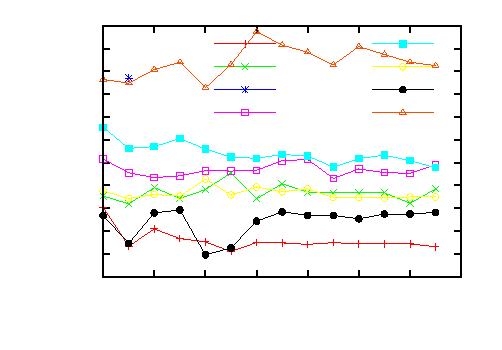
\includegraphics{costsB}}%
    \gplfronttext
  \end{picture}%
\endgroup

\caption{Solutions for the rest of the ITC instances\label{costsB}}
\end{figure}

\subsection{University course scheduling\label{ITC}}

Automated timetabling is nowadays a crucial application, as many educational institutes still use ad hoc manual processes to schedule their courses. The International Time\-ta\-bl\-in\-g Competition (ITC) is an attempt to unify all these processes. We borrowed the fourteen instances of the latest contest track concerning \emph{universities}.\cite{itc-agenda}

In these problems, we have to assign valid teaching periods and rooms to the curriculum lectures. The objective is to distribute them evenly during the week but without having gaps between them, if scheduled on the same day; each gap increases the solution cost.\cite{pothitos-ictai2012}

Due to ITC specifications, we had 333 seconds in our machine to solve each instance and minimize the solution cost as much as we could. Figures \ref{costsA} and \ref{costsB} display the minimum solution costs found per instance by \textsc{PopsSample} for various $\mathsf{conf}$ values. We observe that as $\mathsf{conf}$ increases the costs tend to a specific number, whilst for small $\mathsf{conf}$ values we have fluctuations because search becomes more random.

%In this problem, heuristics help search by choosing (i) the next variable to instantiate and (ii) the value to assign to the variable. In the evaluations, we applied our framework only on phase (i), but for the \textsc{PoPS} experiments in Section~\ref{PoPS} etc.\ we applied it on (ii).

It was expected that for high $\mathsf{conf}$ values the results would be more stable, as the search process approximates the default depth-first-search (DFS). For the marginal low values, e.g.\ $\mathsf{conf} = 0$, search is completely stochastic and the results are worse on overage, as we have higher solution costs. However, the evaluations for intermediate $\mathsf{conf}$ values, e.g.\ $\mathsf{conf} \approx 20$, are more promising, but the automatic selection of the best $\mathsf{conf}$ is an open question here; in the last sections, \textsc{PoPS} finds automatically appropriate $\mathsf{conf}$ values.

In practice, as shown in Fig.\ \ref{costsA} and \ref{costsB}, a $\mathsf{conf}$ value around $100$ actually represents infinity, because search tends to produce the same solutions for $\mathsf{conf} \geq 100$.

It is worth to mention that in Fig.~\ref{costsB} the only solution found for the \textsf{Let0405-1} instance, depicted with an asterisk~\textcolor{blue}{$*$}, was for $\mathsf{conf} = 10$.

\subsection{Radio link frequency assignment}

Another important real problem is the frequency assignment, in which we have to assign a frequency to each radio transmitter with the objective to minimize the interference. The interference is minimized by assigning different frequencies to every two transmitters that are close to each other.

The Centre Electronique de l'Armement (CELAR) provides a set of real datasets for this NP-hard problem.\cite{radio-link} We chose to solve the five so-called ``MAX'' problem instances, namely \textsf{SCEN06}--\textsf{SCEN10}, in which, generally speaking, we try to maximize the number of the satisfied soft constraints.

For each of these instances, we had 15 minutes to explore the search space. We recorded the best (lowest) solution costs found so far in Fig.~\ref{CELAR} for several $\mathsf{conf}$ values. Approximately the same as in course scheduling, the lowest solution costs occur around $\mathsf{conf} \approx 10$, which gives better results on average than the marginal $\mathsf{conf}$ values.

\begin{figure}
\centering
% GNUPLOT: LaTeX picture with Postscript
\begingroup
  \makeatletter
  \providecommand\color[2][]{%
    \GenericError{(gnuplot) \space\space\space\@spaces}{%
      Package color not loaded in conjunction with
      terminal option `colourtext'%
    }{See the gnuplot documentation for explanation.%
    }{Either use 'blacktext' in gnuplot or load the package
      color.sty in LaTeX.}%
    \renewcommand\color[2][]{}%
  }%
  \providecommand\includegraphics[2][]{%
    \GenericError{(gnuplot) \space\space\space\@spaces}{%
      Package graphicx or graphics not loaded%
    }{See the gnuplot documentation for explanation.%
    }{The gnuplot epslatex terminal needs graphicx.sty or graphics.sty.}%
    \renewcommand\includegraphics[2][]{}%
  }%
  \providecommand\rotatebox[2]{#2}%
  \@ifundefined{ifGPcolor}{%
    \newif\ifGPcolor
    \GPcolortrue
  }{}%
  \@ifundefined{ifGPblacktext}{%
    \newif\ifGPblacktext
    \GPblacktexttrue
  }{}%
  % define a \g@addto@macro without @ in the name:
  \let\gplgaddtomacro\g@addto@macro
  % define empty templates for all commands taking text:
  \gdef\gplbacktext{}%
  \gdef\gplfronttext{}%
  \makeatother
  \ifGPblacktext
    % no textcolor at all
    \def\colorrgb#1{}%
    \def\colorgray#1{}%
  \else
    % gray or color?
    \ifGPcolor
      \def\colorrgb#1{\color[rgb]{#1}}%
      \def\colorgray#1{\color[gray]{#1}}%
      \expandafter\def\csname LTw\endcsname{\color{white}}%
      \expandafter\def\csname LTb\endcsname{\color{black}}%
      \expandafter\def\csname LTa\endcsname{\color{black}}%
      \expandafter\def\csname LT0\endcsname{\color[rgb]{1,0,0}}%
      \expandafter\def\csname LT1\endcsname{\color[rgb]{0,1,0}}%
      \expandafter\def\csname LT2\endcsname{\color[rgb]{0,0,1}}%
      \expandafter\def\csname LT3\endcsname{\color[rgb]{1,0,1}}%
      \expandafter\def\csname LT4\endcsname{\color[rgb]{0,1,1}}%
      \expandafter\def\csname LT5\endcsname{\color[rgb]{1,1,0}}%
      \expandafter\def\csname LT6\endcsname{\color[rgb]{0,0,0}}%
      \expandafter\def\csname LT7\endcsname{\color[rgb]{1,0.3,0}}%
      \expandafter\def\csname LT8\endcsname{\color[rgb]{0.5,0.5,0.5}}%
    \else
      % gray
      \def\colorrgb#1{\color{black}}%
      \def\colorgray#1{\color[gray]{#1}}%
      \expandafter\def\csname LTw\endcsname{\color{white}}%
      \expandafter\def\csname LTb\endcsname{\color{black}}%
      \expandafter\def\csname LTa\endcsname{\color{black}}%
      \expandafter\def\csname LT0\endcsname{\color{black}}%
      \expandafter\def\csname LT1\endcsname{\color{black}}%
      \expandafter\def\csname LT2\endcsname{\color{black}}%
      \expandafter\def\csname LT3\endcsname{\color{black}}%
      \expandafter\def\csname LT4\endcsname{\color{black}}%
      \expandafter\def\csname LT5\endcsname{\color{black}}%
      \expandafter\def\csname LT6\endcsname{\color{black}}%
      \expandafter\def\csname LT7\endcsname{\color{black}}%
      \expandafter\def\csname LT8\endcsname{\color{black}}%
    \fi
  \fi
  \setlength{\unitlength}{0.0500bp}%
  \begin{picture}(4750.00,4750.00)%
    \gplgaddtomacro\gplbacktext{%
      \csname LTb\endcsname%
      \put(660,3910){\makebox(0,0)[r]{\strut{}$\scriptstyle{280000}$}}%
      \put(660,4150){\makebox(0,0)[r]{\strut{}$\scriptstyle{300000}$}}%
      \put(660,4389){\makebox(0,0)[r]{\strut{}$\scriptstyle{320000}$}}%
      \put(660,4629){\makebox(0,0)[r]{\strut{}$\scriptstyle{340000}$}}%
      \put(792,3690){\makebox(0,0){\strut{}}}%
      \put(1380,3690){\makebox(0,0){\strut{}}}%
      \put(1969,3690){\makebox(0,0){\strut{}}}%
      \put(2557,3690){\makebox(0,0){\strut{}}}%
      \put(3146,3690){\makebox(0,0){\strut{}}}%
      \put(3734,3690){\makebox(0,0){\strut{}}}%
      \put(4323,3690){\makebox(0,0){\strut{}}}%
      \put(3967,4204){\makebox(0,0)[l]{\strut{}\textsf{\scriptsize SCEN07}}}%
    }%
    \gplgaddtomacro\gplfronttext{%
    }%
    \gplgaddtomacro\gplbacktext{%
      \csname LTb\endcsname%
      \put(660,3100){\makebox(0,0)[r]{\strut{}$\scriptstyle{10000}$}}%
      \put(660,3380){\makebox(0,0)[r]{\strut{}$\scriptstyle{11000}$}}%
      \put(660,3659){\makebox(0,0)[r]{\strut{}$\scriptstyle{12000}$}}%
      \put(792,2740){\makebox(0,0){\strut{}}}%
      \put(1380,2740){\makebox(0,0){\strut{}}}%
      \put(1969,2740){\makebox(0,0){\strut{}}}%
      \put(2557,2740){\makebox(0,0){\strut{}}}%
      \put(3146,2740){\makebox(0,0){\strut{}}}%
      \put(3734,2740){\makebox(0,0){\strut{}}}%
      \put(4323,2740){\makebox(0,0){\strut{}}}%
      \put(3967,3212){\makebox(0,0)[l]{\strut{}\textsf{\scriptsize SCEN10}}}%
    }%
    \gplgaddtomacro\gplfronttext{%
    }%
    \gplgaddtomacro\gplbacktext{%
      \csname LTb\endcsname%
      \put(660,2010){\makebox(0,0)[r]{\strut{}$\scriptstyle{460}$}}%
      \put(660,2220){\makebox(0,0)[r]{\strut{}$\scriptstyle{480}$}}%
      \put(660,2430){\makebox(0,0)[r]{\strut{}$\scriptstyle{500}$}}%
      \put(660,2639){\makebox(0,0)[r]{\strut{}$\scriptstyle{520}$}}%
      \put(660,2849){\makebox(0,0)[r]{\strut{}$\scriptstyle{540}$}}%
      \put(792,1790){\makebox(0,0){\strut{}}}%
      \put(1380,1790){\makebox(0,0){\strut{}}}%
      \put(1969,1790){\makebox(0,0){\strut{}}}%
      \put(2557,1790){\makebox(0,0){\strut{}}}%
      \put(3146,1790){\makebox(0,0){\strut{}}}%
      \put(3734,1790){\makebox(0,0){\strut{}}}%
      \put(4323,1790){\makebox(0,0){\strut{}}}%
      \put(154,2429){\rotatebox{-270}{\makebox(0,0){\strut{}Solution Cost (thousands)}}}%
      \put(3967,2346){\makebox(0,0)[l]{\strut{}\textsf{\scriptsize SCEN09}}}%
    }%
    \gplgaddtomacro\gplfronttext{%
    }%
    \gplgaddtomacro\gplbacktext{%
      \csname LTb\endcsname%
      \put(660,1200){\makebox(0,0)[r]{\strut{}$\scriptstyle{170}$}}%
      \put(660,1480){\makebox(0,0)[r]{\strut{}$\scriptstyle{180}$}}%
      \put(660,1760){\makebox(0,0)[r]{\strut{}$\scriptstyle{190}$}}%
      \put(792,840){\makebox(0,0){\strut{}}}%
      \put(1380,840){\makebox(0,0){\strut{}}}%
      \put(1969,840){\makebox(0,0){\strut{}}}%
      \put(2557,840){\makebox(0,0){\strut{}}}%
      \put(3146,840){\makebox(0,0){\strut{}}}%
      \put(3734,840){\makebox(0,0){\strut{}}}%
      \put(4323,840){\makebox(0,0){\strut{}}}%
      \put(3967,1354){\makebox(0,0)[l]{\strut{}\textsf{\scriptsize SCEN06}}}%
    }%
    \gplgaddtomacro\gplfronttext{%
    }%
    \gplgaddtomacro\gplbacktext{%
      \csname LTb\endcsname%
      \put(660,568){\makebox(0,0)[r]{\strut{}$\scriptstyle{8.4}$}}%
      \put(660,823){\makebox(0,0)[r]{\strut{}$\scriptstyle{8.6}$}}%
      \put(792,220){\makebox(0,0){\strut{}$\scriptstyle{0}$}}%
      \put(1380,220){\makebox(0,0){\strut{}$\scriptstyle{20}$}}%
      \put(1969,220){\makebox(0,0){\strut{}$\scriptstyle{40}$}}%
      \put(2557,220){\makebox(0,0){\strut{}$\scriptstyle{60}$}}%
      \put(3146,220){\makebox(0,0){\strut{}$\scriptstyle{80}$}}%
      \put(3734,220){\makebox(0,0){\strut{}$\scriptstyle{100}$}}%
      \put(4323,220){\makebox(0,0){\strut{}$\scriptstyle{120}$}}%
      \put(2704,-110){\makebox(0,0){\strut{}$\mathsf{conf}$}}%
      \put(3967,823){\makebox(0,0)[l]{\strut{}\textsf{\scriptsize SCEN08}}}%
    }%
    \gplgaddtomacro\gplfronttext{%
    }%
    \gplbacktext
    \put(0,0){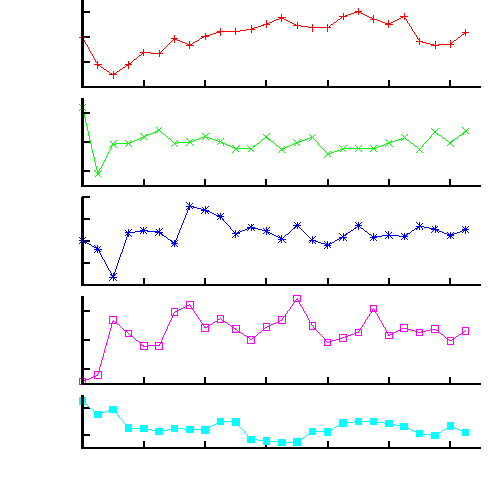
\includegraphics{CELAR}}%
    \gplfronttext
  \end{picture}%
\endgroup

\caption{Unsatisfied soft constraints increase cost\label{CELAR}}
\end{figure}

\subsection{\PopsSample{} during hard optimization\label{PoPS}}

The $\mathsf{conf}$ parameter can refine any search method that adopts our heuristic framework. The \textsc{PopsSample} method goes a step further: it incorporates our heuristic \emph{confidence semantics} into its search engine.

In order to solve the first university course timetabling instance (\textsf{Fis0506-1} of Section~\ref{ITC}), we invoked \textsc{PopsSample} for various $\mathsf{PieceToCover}$ and $\mathsf{conf}$ values and we plotted the best solution costs found in Figure~\ref{ITC1}. The third dimension is the $cost$ of the solutions found: the lower the solution cost is, the more qualitative timetable is produced.

\begin{figure}
\centering
% GNUPLOT: LaTeX picture with Postscript
\begingroup
  \makeatletter
  \providecommand\color[2][]{%
    \GenericError{(gnuplot) \space\space\space\@spaces}{%
      Package color not loaded in conjunction with
      terminal option `colourtext'%
    }{See the gnuplot documentation for explanation.%
    }{Either use 'blacktext' in gnuplot or load the package
      color.sty in LaTeX.}%
    \renewcommand\color[2][]{}%
  }%
  \providecommand\includegraphics[2][]{%
    \GenericError{(gnuplot) \space\space\space\@spaces}{%
      Package graphicx or graphics not loaded%
    }{See the gnuplot documentation for explanation.%
    }{The gnuplot epslatex terminal needs graphicx.sty or graphics.sty.}%
    \renewcommand\includegraphics[2][]{}%
  }%
  \providecommand\rotatebox[2]{#2}%
  \@ifundefined{ifGPcolor}{%
    \newif\ifGPcolor
    \GPcolortrue
  }{}%
  \@ifundefined{ifGPblacktext}{%
    \newif\ifGPblacktext
    \GPblacktexttrue
  }{}%
  % define a \g@addto@macro without @ in the name:
  \let\gplgaddtomacro\g@addto@macro
  % define empty templates for all commands taking text:
  \gdef\gplbacktext{}%
  \gdef\gplfronttext{}%
  \makeatother
  \ifGPblacktext
    % no textcolor at all
    \def\colorrgb#1{}%
    \def\colorgray#1{}%
  \else
    % gray or color?
    \ifGPcolor
      \def\colorrgb#1{\color[rgb]{#1}}%
      \def\colorgray#1{\color[gray]{#1}}%
      \expandafter\def\csname LTw\endcsname{\color{white}}%
      \expandafter\def\csname LTb\endcsname{\color{black}}%
      \expandafter\def\csname LTa\endcsname{\color{black}}%
      \expandafter\def\csname LT0\endcsname{\color[rgb]{1,0,0}}%
      \expandafter\def\csname LT1\endcsname{\color[rgb]{0,1,0}}%
      \expandafter\def\csname LT2\endcsname{\color[rgb]{0,0,1}}%
      \expandafter\def\csname LT3\endcsname{\color[rgb]{1,0,1}}%
      \expandafter\def\csname LT4\endcsname{\color[rgb]{0,1,1}}%
      \expandafter\def\csname LT5\endcsname{\color[rgb]{1,1,0}}%
      \expandafter\def\csname LT6\endcsname{\color[rgb]{0,0,0}}%
      \expandafter\def\csname LT7\endcsname{\color[rgb]{1,0.3,0}}%
      \expandafter\def\csname LT8\endcsname{\color[rgb]{0.5,0.5,0.5}}%
    \else
      % gray
      \def\colorrgb#1{\color{black}}%
      \def\colorgray#1{\color[gray]{#1}}%
      \expandafter\def\csname LTw\endcsname{\color{white}}%
      \expandafter\def\csname LTb\endcsname{\color{black}}%
      \expandafter\def\csname LTa\endcsname{\color{black}}%
      \expandafter\def\csname LT0\endcsname{\color{black}}%
      \expandafter\def\csname LT1\endcsname{\color{black}}%
      \expandafter\def\csname LT2\endcsname{\color{black}}%
      \expandafter\def\csname LT3\endcsname{\color{black}}%
      \expandafter\def\csname LT4\endcsname{\color{black}}%
      \expandafter\def\csname LT5\endcsname{\color{black}}%
      \expandafter\def\csname LT6\endcsname{\color{black}}%
      \expandafter\def\csname LT7\endcsname{\color{black}}%
      \expandafter\def\csname LT8\endcsname{\color{black}}%
    \fi
  \fi
  \setlength{\unitlength}{0.0500bp}%
  \begin{picture}(4824.00,3376.80)%
    \gplgaddtomacro\gplbacktext{%
      \csname LTb\endcsname%
      \put(3970,2058){\makebox(0,0)[l]{\strut{}\textcolor{green}{DFS}}}%
      \put(3970,1851){\makebox(0,0)[l]{\strut{}\textcolor{cyan}{Iterative}}}%
      \put(3970,1677){\makebox(0,0)[l]{\strut{}\textcolor{cyan}{Broadening}}}%
      \put(3970,1414){\makebox(0,0)[l]{\strut{}\textcolor{orange}{LDS}}}%
      \put(450,913){\rotatebox{-15}{\makebox(0,0)[l]{\strut{}$\mathsf{PieceToCover}$}}}%
    }%
    \gplgaddtomacro\gplfronttext{%
      \csname LTb\endcsname%
      \put(1612,838){\makebox(0,0)[r]{\strut{}$\scriptstyle{0}$}}%
      \put(1205,954){\makebox(0,0)[r]{\strut{}$\scriptstyle{0.5}$}}%
      \put(798,1071){\makebox(0,0)[r]{\strut{}$\scriptstyle{1}$}}%
      \put(3983,958){\makebox(0,0){\strut{}$\scriptstyle{0}$}}%
      \put(3663,946){\makebox(0,0){\strut{}$\scriptstyle{20}$}}%
      \put(3344,934){\makebox(0,0){\strut{}$\scriptstyle{40}$}}%
      \put(3024,922){\makebox(0,0){\strut{}$\scriptstyle{60}$}}%
      \put(2704,910){\makebox(0,0){\strut{}$\scriptstyle{80}$}}%
      \put(2385,898){\makebox(0,0){\strut{}$\scriptstyle{100}$}}%
      \put(2066,886){\makebox(0,0){\strut{}$\scriptstyle{120}$}}%
      \put(1746,874){\makebox(0,0){\strut{}$\scriptstyle{140}$}}%
      \put(2866,659){\makebox(0,0){\strut{}$\mathsf{conf}$}}%
      \put(760,1171){\makebox(0,0)[r]{\strut{}$\scriptstyle{50}$}}%
      \put(760,1346){\makebox(0,0)[r]{\strut{}$\scriptstyle{100}$}}%
      \put(760,1522){\makebox(0,0)[r]{\strut{}$\scriptstyle{150}$}}%
      \put(760,1697){\makebox(0,0)[r]{\strut{}$\scriptstyle{200}$}}%
      \put(760,1871){\makebox(0,0)[r]{\strut{}$\scriptstyle{250}$}}%
      \put(760,2047){\makebox(0,0)[r]{\strut{}$\scriptstyle{300}$}}%
      \put(760,2222){\makebox(0,0)[r]{\strut{}$\scriptstyle{350}$}}%
      \put(760,2398){\makebox(0,0)[r]{\strut{}$\scriptstyle{400}$}}%
      \put(760,2573){\makebox(0,0)[r]{\strut{}$\scriptstyle{450}$}}%
      \put(358,1871){\rotatebox{-270}{\makebox(0,0){\strut{}Solution Cost}}}%
    }%
    \gplbacktext
    \put(0,0){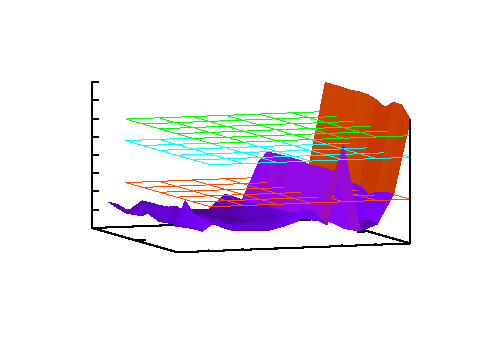
\includegraphics{ITC1}}%
    \gplfronttext
  \end{picture}%
\endgroup

\caption{{\normalfont\textsc{PopsSample}} for the first ITC instance\label{ITC1}}
\end{figure}

In the same graphs we include some of the well-known search methods results, such as DFS, LDS, and Iterative Broadening, implementesd in the same solver, with only their best solution cost depicted as a plane grid, in order to make comparisons easily.

%In the first two instances, \textsc{PoPS} outperforms the other systematic search methods. In the third instance \textsc{PoPS} comes second to DBS, but approximates it; generally speaking, with regard to the rest of the instances, the best parameters for \textsc{PoPS} are inside the area around the spot $(\mathsf{PieceToCover}, \mathsf{conf}) = (60, 0.4)$.

\subsection{\PoPS{} vs.\ other search methods}

In the above sections, it was not easy to figure out which is the best $\mathsf{PieceToCover}$ and $\mathsf{conf}$ combination. That is why we employed \textsc{PoPS} to solve the fourteen course timetabling instances. As described in Section~\ref{sampling}, \textsc{PoPS} uses several $\mathsf{conf}$ values and favours the most fruitful ones. We used five $\mathsf{conf}$ samples, i.e.\ $0$, $25$, $50$, $75$, and $100$, by setting $\mathsf{SamplesNum}$ equal to $5$. In this way, \textsc{PoPS} constructed solutions with lower costs than the other methods, except for the fifth instance, as illustrated in Table~\ref{PopsItc}. The time limit for all the methods was set to 15 minutes.

\begin{table}
\centering
\caption{Solution costs for fourteen ITC instances\label{PopsItc}}
\begin{tabular}{|c|c|c|c|c|}
\hline
                      Instance & PoPS & LDS & DFS & It.\ Broad. \\
\hline
\hline
\textsf{Fis0506-1} &  $\mathit{105}$ & $171$ & $345$ & $286$  \\ \hline
\textsf{Ing0203-2} &  $\mathit{241}$ & $288$ & $698$ & $321$  \\ \hline
\textsf{Ing0304-1} &  $\mathit{279}$ & $307$ & $578$ & $353$  \\ \hline
\textsf{Ing0405-3} &  $\mathit{195}$ & $215$ & $817$ & $235$  \\ \hline
\textsf{Let0405-1} &  $655$ & $\mathit{627}$ & X & X          \\ \hline
\textsf{Ing0506-1} &  $\mathit{307}$ & $311$ & $812$ & $342$  \\ \hline
\textsf{Ing0607-2} &  $\mathit{282}$ & $283$ & $1184$ & $328$ \\ \hline
\textsf{Ing0607-3} &  $\mathit{223}$ & $239$ & $635$ & $262$  \\ \hline
\textsf{Ing0304-3} &  $\mathit{288}$ & $294$ & $675$ & $370$  \\ \hline
\textsf{Ing0405-2} &  $\mathit{265}$ & $284$ & $877$ & $344$  \\ \hline
\textsf{Fis0506-2} &  $\mathit{12}$ & $33$ & $486$ & $34$     \\ \hline
\textsf{Let0506-2} &  $\mathit{713}$ & $783$ & $1621$ & $937$ \\ \hline
\textsf{Ing0506-3} &  $\mathit{231}$ & $256$ & $660$ & $280$  \\ \hline
\textsf{Ing0708-1} &  $\mathit{223}$ & $227$ & $660$ & $264$  \\ \hline
\end{tabular}
\end{table}


\section{Conclusions and Perspectives}

We presented a well-founded framework to exploit both stochastic and deterministic heuristics. Empirical evaluations showed that our hybrid approach can produce better results than fully random or fully deterministic methodologies.

%In this context, we introduced a randomness degree value, namely $\mathsf{conf}$, we theoretically founded its semantics, and we linked it with the heuristic \emph{reliability} notion.

In order to achieve this, we approached and used heuristics as a \emph{confidence} and \emph{reliability} measure. By exploiting these heuristic semantics, we were able to produce a new efficient search method, namely \textsc{PoPS}, that can outperform other methodologies. In general, our proposed framework gives the opportunity to exploit ``on the fly'' whichever heuristic confidence fluctuations occur.

In future, it will be challenging to parallelize it, as it supports a whole grid of strategies, by concurrently invoking \textsc{PopsSample} with several $\mathsf{PieceToCover}$ and $\mathsf{conf}$ arguments.

%\begin{figure}
%\centering
%\input{figures/PoPS/ITC2}
%\caption{\textsc{PoPS}$(\mathsf{PieceToCover})$ costs for the second ITC instance\label{ITC2}}
%\end{figure}

%\begin{figure}
%\centering
%\input{figures/PoPS/ITC3}
%\caption{\textsc{PoPS}$(\mathsf{PieceToCover})$ solution costs for the third ITC instance\label{ITC3}}
%\end{figure}

% TODOs %
% Many random trials/seeds
% Compare to HBSS
% Test different heuristics

% Extended LDS %
% A Novel Insight on Defining Search Methods and Incorporating Heuristics
% Keywords: discrepancy, LDS, DDS, heuristic linearization, CSP, constraint programming.

% Template
%\begin{table}
%\tbl{TODO}
%{\begin{tabular}{@{}cccc@{}} \toprule
%Piston Mass & (Rad/s) & (Rad/s) & \% Error \\ \colrule
%0.01\hphantom{0} & 2441.0 & 2441.0\hphantom{0} & 0.0\hphantom{0} \\
%0.001 & 4130.0 & 4129.3\hphantom{0} & 0.16\\ \botrule
%\end{tabular}}
%\end{table}


\section*{Acknowledgments}

We want to thank Foivos Theocharis who initially built the search methods library \textsc{Amorgos}, which is available together with \textsc{Naxos}.\cite{naxos-solver}

\bibliographystyle{ws-ijait}
\bibliography{bibliography}

\end{document}
